\documentclass[twoside]{book}

% Packages required by doxygen
\usepackage{fixltx2e}
\usepackage{calc}
\usepackage{doxygen}
\usepackage[export]{adjustbox} % also loads graphicx
\usepackage{graphicx}
\usepackage[utf8]{inputenc}
\usepackage{makeidx}
\usepackage{multicol}
\usepackage{multirow}
\PassOptionsToPackage{warn}{textcomp}
\usepackage{textcomp}
\usepackage[nointegrals]{wasysym}
\usepackage[table]{xcolor}

% Font selection
\usepackage[T1]{fontenc}
\usepackage[scaled=.90]{helvet}
\usepackage{courier}
\usepackage{amssymb}
\usepackage{sectsty}
\renewcommand{\familydefault}{\sfdefault}
\allsectionsfont{%
  \fontseries{bc}\selectfont%
  \color{darkgray}%
}
\renewcommand{\DoxyLabelFont}{%
  \fontseries{bc}\selectfont%
  \color{darkgray}%
}
\newcommand{\+}{\discretionary{\mbox{\scriptsize$\hookleftarrow$}}{}{}}

% Page & text layout
\usepackage{geometry}
\geometry{%
  a4paper,%
  top=2.5cm,%
  bottom=2.5cm,%
  left=2.5cm,%
  right=2.5cm%
}
\tolerance=750
\hfuzz=15pt
\hbadness=750
\setlength{\emergencystretch}{15pt}
\setlength{\parindent}{0cm}
\setlength{\parskip}{3ex plus 2ex minus 2ex}
\makeatletter
\renewcommand{\paragraph}{%
  \@startsection{paragraph}{4}{0ex}{-1.0ex}{1.0ex}{%
    \normalfont\normalsize\bfseries\SS@parafont%
  }%
}
\renewcommand{\subparagraph}{%
  \@startsection{subparagraph}{5}{0ex}{-1.0ex}{1.0ex}{%
    \normalfont\normalsize\bfseries\SS@subparafont%
  }%
}
\makeatother

% Headers & footers
\usepackage{fancyhdr}
\pagestyle{fancyplain}
\fancyhead[LE]{\fancyplain{}{\bfseries\thepage}}
\fancyhead[CE]{\fancyplain{}{}}
\fancyhead[RE]{\fancyplain{}{\bfseries\leftmark}}
\fancyhead[LO]{\fancyplain{}{\bfseries\rightmark}}
\fancyhead[CO]{\fancyplain{}{}}
\fancyhead[RO]{\fancyplain{}{\bfseries\thepage}}
\fancyfoot[LE]{\fancyplain{}{}}
\fancyfoot[CE]{\fancyplain{}{}}
\fancyfoot[RE]{\fancyplain{}{\bfseries\scriptsize Generated by Doxygen }}
\fancyfoot[LO]{\fancyplain{}{\bfseries\scriptsize Generated by Doxygen }}
\fancyfoot[CO]{\fancyplain{}{}}
\fancyfoot[RO]{\fancyplain{}{}}
\renewcommand{\footrulewidth}{0.4pt}
\renewcommand{\chaptermark}[1]{%
  \markboth{#1}{}%
}
\renewcommand{\sectionmark}[1]{%
  \markright{\thesection\ #1}%
}

% Indices & bibliography
\usepackage{natbib}
\usepackage[titles]{tocloft}
\setcounter{tocdepth}{3}
\setcounter{secnumdepth}{5}
\makeindex

% Custom commands
\newcommand{\clearemptydoublepage}{%
  \newpage{\pagestyle{empty}\cleardoublepage}%
}

\usepackage{caption}
\captionsetup{labelsep=space,justification=centering,font={bf},singlelinecheck=off,skip=4pt,position=top}

%===== C O N T E N T S =====

\begin{document}

% Titlepage & ToC
\pagenumbering{alph}
\begin{titlepage}
\vspace*{7cm}
\begin{center}%
{\Large Firmware documentation -\/ I\+MU board }\\
\vspace*{1cm}
{\large Generated by Doxygen 1.8.13}\\
\end{center}
\end{titlepage}
\clearemptydoublepage
\pagenumbering{roman}
\tableofcontents
\clearemptydoublepage
\pagenumbering{arabic}

%--- Begin generated contents ---
\chapter{Firmware}
\label{index}This is the firmware of the I\+MU board. \begin{DoxyVersion}{Version}
1.\+0
\end{DoxyVersion}
This is the firmware of the I\+MU board. It can read up to 17 I\+MU modules connected to the P\+SoC microcontroller. 
\chapter{Data Structure Index}
\section{Data Structures}
Here are the data structures with brief descriptions\+:\begin{DoxyCompactList}
\item\contentsline{section}{\textbf{ st\+\_\+data} }{\pageref{structst__data}}{}
\item\contentsline{section}{\textbf{ st\+\_\+imu} }{\pageref{structst__imu}}{}
\item\contentsline{section}{\textbf{ st\+\_\+mem} }{\pageref{structst__mem}}{}
\end{DoxyCompactList}

\chapter{File Index}
\section{File List}
Here is a list of all documented files with brief descriptions\+:\begin{DoxyCompactList}
\item\contentsline{section}{\textbf{ command\+\_\+processing.\+c} \\*Command processing functions }{\pageref{command__processing_8c}}{}
\item\contentsline{section}{\textbf{ command\+\_\+processing.\+h} \\*Definition of command processing functions }{\pageref{command__processing_8h}}{}
\item\contentsline{section}{\textbf{ commands.\+h} \\*Definitions for commands, parameters and packages }{\pageref{commands_8h}}{}
\item\contentsline{section}{{\bfseries device.\+h} }{\pageref{device_8h}}{}
\item\contentsline{section}{\textbf{ globals.\+c} \\*Global variables }{\pageref{globals_8c}}{}
\item\contentsline{section}{\textbf{ globals.\+h} \\*Global definitions and macros are set in this file }{\pageref{globals_8h}}{}
\item\contentsline{section}{\textbf{ I\+M\+U\+\_\+functions.\+c} \\*Implementation of I\+MU module functions }{\pageref{_i_m_u__functions_8c}}{}
\item\contentsline{section}{\textbf{ I\+M\+U\+\_\+functions.\+h} \\*Definition of I\+MU module functions }{\pageref{_i_m_u__functions_8h}}{}
\item\contentsline{section}{\textbf{ interruptions.\+c} \\*Interruption functions are in this file }{\pageref{interruptions_8c}}{}
\item\contentsline{section}{\textbf{ interruptions.\+h} \\*Interruptions header file }{\pageref{interruptions_8h}}{}
\item\contentsline{section}{\textbf{ main.\+c} \\*Firmware main file }{\pageref{main_8c}}{}
\item\contentsline{section}{\textbf{ utils.\+h} \\*Definition of utility functions }{\pageref{utils_8h}}{}
\end{DoxyCompactList}

\chapter{Data Structure Documentation}
\section{st\+\_\+data Struct Reference}
\label{structst__data}\index{st\+\_\+data@{st\+\_\+data}}
\subsection*{Data Fields}
\begin{DoxyCompactItemize}
\item 
\mbox{\label{structst__data_ae690fc5f3d08456a861f43937912613d}} 
uint8 {\bfseries buffer} [128]
\item 
\mbox{\label{structst__data_a3fb0e45fa764ccedd2dd8c0654c2e743}} 
int16 {\bfseries length}
\item 
\mbox{\label{structst__data_a5d76dba8ca72d027d149ffcf8760f2ca}} 
int16 {\bfseries ind}
\item 
\mbox{\label{structst__data_ac24f07ab21d61d7af9cb3a49d102e0ac}} 
uint8 {\bfseries ready}
\end{DoxyCompactItemize}


The documentation for this struct was generated from the following file\+:\begin{DoxyCompactItemize}
\item 
\textbf{ globals.\+h}\end{DoxyCompactItemize}

\section{st\+\_\+imu Struct Reference}
\label{structst__imu}\index{st\+\_\+imu@{st\+\_\+imu}}
\subsection*{Data Fields}
\begin{DoxyCompactItemize}
\item 
\mbox{\label{structst__imu_acd8859336a5cb8a70051c97a438726a1}} 
uint8 {\bfseries flags}
\item 
\mbox{\label{structst__imu_a76e9575b13f4c390ccec733a5dac028f}} 
int16 {\bfseries accel\+\_\+value} [3]
\item 
\mbox{\label{structst__imu_a515e671f6e4fe912e9af6c73a8d654b9}} 
int16 {\bfseries gyro\+\_\+value} [3]
\item 
\mbox{\label{structst__imu_ae78e11a5f5ad413f738f6eb69ac60277}} 
int16 {\bfseries mag\+\_\+value} [3]
\item 
\mbox{\label{structst__imu_a2825af9e90a3b4d11e0f99f34a73d555}} 
float {\bfseries quat\+\_\+value} [4]
\item 
\mbox{\label{structst__imu_a093731ce8df43a5beb8df6e78368ec4c}} 
int16 {\bfseries temp\+\_\+value}
\end{DoxyCompactItemize}


The documentation for this struct was generated from the following file\+:\begin{DoxyCompactItemize}
\item 
\textbf{ globals.\+h}\end{DoxyCompactItemize}

\section{st\+\_\+mem Struct Reference}
\label{structst__mem}\index{st\+\_\+mem@{st\+\_\+mem}}
\subsection*{Data Fields}
\begin{DoxyCompactItemize}
\item 
\mbox{\label{structst__mem_af11e40d15a1361229a78e772af5b3c94}} 
uint8 {\bfseries flag}
\item 
\mbox{\label{structst__mem_a492bfda30c3852a68b2cbfba9531e3d1}} 
uint8 {\bfseries id}
\item 
\mbox{\label{structst__mem_a1a2b3002580421effeca67955a862580}} 
uint8 {\bfseries baud\+\_\+rate}
\item 
\mbox{\label{structst__mem_aa5b15dee0878926cf86de9d3a70d3b30}} 
uint8 {\bfseries S\+P\+I\+\_\+read\+\_\+delay}
\item 
\mbox{\label{structst__mem_a14af68f87b94c84ebf2d503396b4aa47}} 
uint8 {\bfseries I\+M\+U\+\_\+conf} [N\+\_\+\+I\+M\+U\+\_\+\+M\+AX][N\+U\+M\+\_\+\+O\+F\+\_\+\+D\+A\+TA]
\end{DoxyCompactItemize}


The documentation for this struct was generated from the following file\+:\begin{DoxyCompactItemize}
\item 
\textbf{ globals.\+h}\end{DoxyCompactItemize}

\chapter{File Documentation}
\section{command\+\_\+processing.\+c File Reference}
\label{command__processing_8c}\index{command\+\_\+processing.\+c@{command\+\_\+processing.\+c}}


Command processing functions.  


{\ttfamily \#include \char`\"{}command\+\_\+processing.\+h\char`\"{}}\newline
{\ttfamily \#include \char`\"{}interruptions.\+h\char`\"{}}\newline
{\ttfamily \#include \char`\"{}utils.\+h\char`\"{}}\newline
{\ttfamily \#include \char`\"{}globals.\+h\char`\"{}}\newline
{\ttfamily \#include \char`\"{}commands.\+h\char`\"{}}\newline
{\ttfamily \#include \char`\"{}I\+M\+U\+\_\+functions.\+h\char`\"{}}\newline
{\ttfamily \#include $<$S\+T\+D\+I\+O.\+H$>$}\newline
Include dependency graph for command\+\_\+processing.\+c\+:
\nopagebreak
\begin{figure}[H]
\begin{center}
\leavevmode
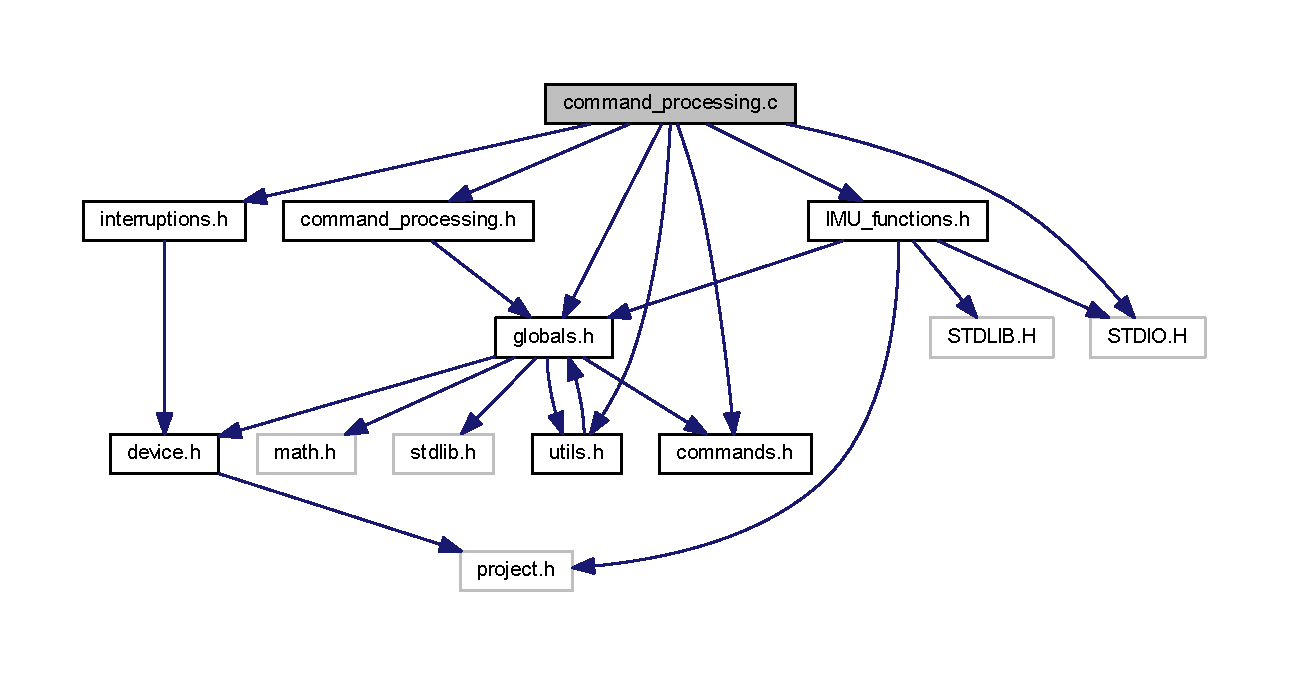
\includegraphics[width=350pt]{command__processing_8c__incl}
\end{center}
\end{figure}
\subsection*{Functions}
\begin{DoxyCompactItemize}
\item 
\mbox{\label{command__processing_8c_a2e5d1711e19837adc3e8f479af3ae509}} 
void {\bfseries comm\+Process} ()
\item 
\mbox{\label{command__processing_8c_af5dcf9e6d2a6421fbe636487e7f9f240}} 
void {\bfseries info\+Send} ()
\item 
\mbox{\label{command__processing_8c_a525ccbc7ac3901d938dc352172ee2531}} 
void {\bfseries info\+Get} (uint16 info\+\_\+type)
\item 
\mbox{\label{command__processing_8c_a5ef086c932682ca5f7549b74ead732aa}} 
void {\bfseries get\+\_\+param\+\_\+list} (uint16 index)
\item 
\mbox{\label{command__processing_8c_abacf855ed80e3052a5bb5b243a0d809e}} 
void {\bfseries info\+Prepare} (unsigned char $\ast$info\+\_\+string)
\item 
\mbox{\label{command__processing_8c_a6762f8be034e0cc6e89e468480242a98}} 
void {\bfseries info\+Reading} (unsigned char $\ast$info\+\_\+string)
\item 
\mbox{\label{command__processing_8c_a49ef41d195291783b6c0e25a0da21a84}} 
void {\bfseries comm\+Write} (uint8 $\ast$packet\+\_\+data, const uint16 packet\+\_\+lenght)
\item 
\mbox{\label{command__processing_8c_a6205a6e88f72f4cc321a7d8abca23e26}} 
uint8 {\bfseries L\+C\+R\+Checksum} (uint8 $\ast$data\+\_\+array, uint8 data\+\_\+length)
\item 
\mbox{\label{command__processing_8c_af4a42b25376d2efd09096cbbed2fbce4}} 
void {\bfseries send\+Acknowledgment} (const uint8 value)
\item 
uint8 \textbf{ mem\+Store} (int displacement)
\item 
void \textbf{ mem\+Recall} ()
\item 
uint8 \textbf{ mem\+Restore} ()
\item 
uint8 \textbf{ mem\+Init} ()
\item 
void \textbf{ cmd\+\_\+set\+\_\+baudrate} ()
\item 
\mbox{\label{command__processing_8c_a704f8c8cb0f4d75f243fc2b79bc34188}} 
void {\bfseries cmd\+\_\+ping} ()
\item 
\mbox{\label{command__processing_8c_a1a2493bfc2f30171d7e7a3bd5aebab14}} 
void {\bfseries cmd\+\_\+store\+\_\+params} ()
\item 
\mbox{\label{command__processing_8c_a40f7c67690279132ab72019b76165cb8}} 
void {\bfseries cmd\+\_\+get\+\_\+imu\+\_\+readings} ()
\end{DoxyCompactItemize}
\subsection*{Variables}
\begin{DoxyCompactItemize}
\item 
\mbox{\label{command__processing_8c_aba5b9353e6d38cc61eb2bd363df61248}} 
reg8 $\ast$ {\bfseries E\+E\+P\+R\+O\+M\+\_\+\+A\+D\+DR} = (reg8 $\ast$) C\+Y\+D\+E\+V\+\_\+\+E\+E\+\_\+\+B\+A\+SE
\end{DoxyCompactItemize}


\subsection{Detailed Description}
Command processing functions. 

\begin{DoxyDate}{Date}
February 01, 2018 
\end{DoxyDate}
\begin{DoxyAuthor}{Author}
{\itshape Centro \char`\"{}\+E.\+Piaggio\char`\"{}} 
\end{DoxyAuthor}
\begin{DoxyCopyright}{Copyright}
(C) 2012-\/2016 qbrobotics. All rights reserved. 

(C) 2017-\/2018 Centro \char`\"{}\+E.\+Piaggio\char`\"{}. All rights reserved. 
\end{DoxyCopyright}


\subsection{Function Documentation}
\mbox{\label{command__processing_8c_aa86bf1f2fa69ab5927f7e4e40eb40581}} 
\index{command\+\_\+processing.\+c@{command\+\_\+processing.\+c}!cmd\+\_\+set\+\_\+baudrate@{cmd\+\_\+set\+\_\+baudrate}}
\index{cmd\+\_\+set\+\_\+baudrate@{cmd\+\_\+set\+\_\+baudrate}!command\+\_\+processing.\+c@{command\+\_\+processing.\+c}}
\subsubsection{cmd\+\_\+set\+\_\+baudrate()}
{\footnotesize\ttfamily void cmd\+\_\+set\+\_\+baudrate (\begin{DoxyParamCaption}{ }\end{DoxyParamCaption})}

Bunch of functions used on request from U\+A\+RT communication \mbox{\label{command__processing_8c_afe52941f8bc21271e811fb0d9f265f38}} 
\index{command\+\_\+processing.\+c@{command\+\_\+processing.\+c}!mem\+Init@{mem\+Init}}
\index{mem\+Init@{mem\+Init}!command\+\_\+processing.\+c@{command\+\_\+processing.\+c}}
\subsubsection{mem\+Init()}
{\footnotesize\ttfamily uint8 mem\+Init (\begin{DoxyParamCaption}{ }\end{DoxyParamCaption})}

This function initialize memory when eeprom is compromised. \mbox{\label{command__processing_8c_a3d3b232874d20b4317e9a79cc3c328d9}} 
\index{command\+\_\+processing.\+c@{command\+\_\+processing.\+c}!mem\+Recall@{mem\+Recall}}
\index{mem\+Recall@{mem\+Recall}!command\+\_\+processing.\+c@{command\+\_\+processing.\+c}}
\subsubsection{mem\+Recall()}
{\footnotesize\ttfamily void mem\+Recall (\begin{DoxyParamCaption}{ }\end{DoxyParamCaption})}

This function loads user settings from the eeprom. \mbox{\label{command__processing_8c_abdb69a74e3147f28d6cbd2b1d406c8a9}} 
\index{command\+\_\+processing.\+c@{command\+\_\+processing.\+c}!mem\+Restore@{mem\+Restore}}
\index{mem\+Restore@{mem\+Restore}!command\+\_\+processing.\+c@{command\+\_\+processing.\+c}}
\subsubsection{mem\+Restore()}
{\footnotesize\ttfamily uint8 mem\+Restore (\begin{DoxyParamCaption}{ }\end{DoxyParamCaption})}

This function loads default settings from the eeprom. \mbox{\label{command__processing_8c_a81e6b73c0ee52661736a97c08bdb262b}} 
\index{command\+\_\+processing.\+c@{command\+\_\+processing.\+c}!mem\+Store@{mem\+Store}}
\index{mem\+Store@{mem\+Store}!command\+\_\+processing.\+c@{command\+\_\+processing.\+c}}
\subsubsection{mem\+Store()}
{\footnotesize\ttfamily uint8 mem\+Store (\begin{DoxyParamCaption}\item[{int}]{displacement }\end{DoxyParamCaption})}

This function stores current memory settings on the eeprom with the specified displacement 
\section{command\+\_\+processing.\+h File Reference}
\label{command__processing_8h}\index{command\+\_\+processing.\+h@{command\+\_\+processing.\+h}}


Definition of command processing functions.  


{\ttfamily \#include \char`\"{}globals.\+h\char`\"{}}\newline
Include dependency graph for command\+\_\+processing.\+h\+:
\nopagebreak
\begin{figure}[H]
\begin{center}
\leavevmode
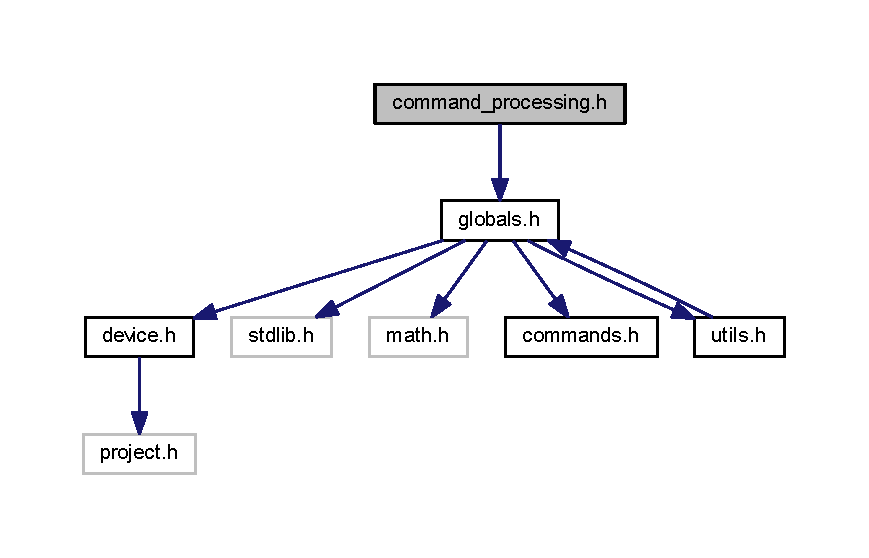
\includegraphics[width=350pt]{command__processing_8h__incl}
\end{center}
\end{figure}
This graph shows which files directly or indirectly include this file\+:
\nopagebreak
\begin{figure}[H]
\begin{center}
\leavevmode
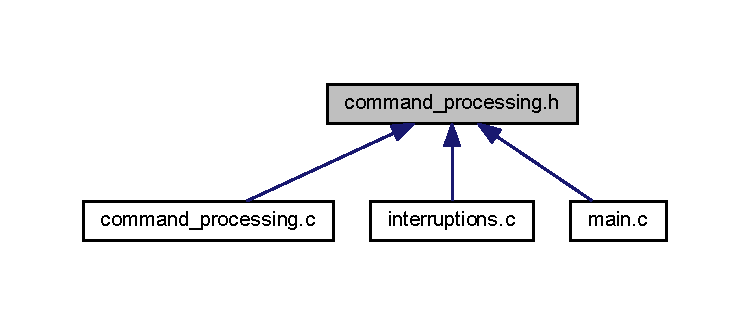
\includegraphics[width=350pt]{command__processing_8h__dep__incl}
\end{center}
\end{figure}
\subsection*{Functions}
\begin{DoxyCompactItemize}
\item 
\mbox{\label{command__processing_8h_a5ef086c932682ca5f7549b74ead732aa}} 
void {\bfseries get\+\_\+param\+\_\+list} (uint16 index)
\item 
\mbox{\label{command__processing_8h_a6fda7bc0be24d261f9cb09e77616b1be}} 
void {\bfseries info\+Prepare} (unsigned char $\ast$)
\item 
\mbox{\label{command__processing_8h_a065ff61e3097bf916aea076a8decb92b}} 
void {\bfseries info\+Reading} (unsigned char $\ast$)
\item 
\mbox{\label{command__processing_8h_af5dcf9e6d2a6421fbe636487e7f9f240}} 
void {\bfseries info\+Send} ()
\item 
\mbox{\label{command__processing_8h_a813734e69ea461791f84bddee422013f}} 
void {\bfseries info\+Get} (uint16)
\item 
\mbox{\label{command__processing_8h_a2e5d1711e19837adc3e8f479af3ae509}} 
void {\bfseries comm\+Process} ()
\item 
\mbox{\label{command__processing_8h_adeaad7a3965fdcfe78aa89533f1ebf39}} 
void {\bfseries comm\+Write} (uint8 $\ast$, const uint16)
\item 
uint8 \textbf{ mem\+Store} (int)
\item 
\mbox{\label{command__processing_8h_afe5c87f9df9bb965976b5d40c4159f1f}} 
void {\bfseries send\+Acknowledgment} (const uint8)
\item 
void \textbf{ mem\+Recall} ()
\item 
uint8 \textbf{ mem\+Restore} ()
\item 
uint8 \textbf{ mem\+Init} ()
\item 
\mbox{\label{command__processing_8h_a6e19f1d501b0105e925c376d93f06a70}} 
uint8 {\bfseries L\+C\+R\+Checksum} (uint8 $\ast$, uint8)
\item 
void \textbf{ cmd\+\_\+set\+\_\+baudrate} ()
\item 
\mbox{\label{command__processing_8h_a1a2493bfc2f30171d7e7a3bd5aebab14}} 
void {\bfseries cmd\+\_\+store\+\_\+params} ()
\item 
\mbox{\label{command__processing_8h_a704f8c8cb0f4d75f243fc2b79bc34188}} 
void {\bfseries cmd\+\_\+ping} ()
\item 
\mbox{\label{command__processing_8h_a40f7c67690279132ab72019b76165cb8}} 
void {\bfseries cmd\+\_\+get\+\_\+imu\+\_\+readings} ()
\end{DoxyCompactItemize}


\subsection{Detailed Description}
Definition of command processing functions. 

\begin{DoxyDate}{Date}
February 01, 2018 
\end{DoxyDate}
\begin{DoxyAuthor}{Author}
{\itshape Centro \char`\"{}\+E.\+Piaggio\char`\"{}} 
\end{DoxyAuthor}
\begin{DoxyCopyright}{Copyright}
(C) 2012-\/2016 qbrobotics. All rights reserved. 

(C) 2017-\/2018 Centro \char`\"{}\+E.\+Piaggio\char`\"{}. All rights reserved. 
\end{DoxyCopyright}


\subsection{Function Documentation}
\mbox{\label{command__processing_8h_aa86bf1f2fa69ab5927f7e4e40eb40581}} 
\index{command\+\_\+processing.\+h@{command\+\_\+processing.\+h}!cmd\+\_\+set\+\_\+baudrate@{cmd\+\_\+set\+\_\+baudrate}}
\index{cmd\+\_\+set\+\_\+baudrate@{cmd\+\_\+set\+\_\+baudrate}!command\+\_\+processing.\+h@{command\+\_\+processing.\+h}}
\subsubsection{cmd\+\_\+set\+\_\+baudrate()}
{\footnotesize\ttfamily void cmd\+\_\+set\+\_\+baudrate (\begin{DoxyParamCaption}{ }\end{DoxyParamCaption})}

Bunch of functions used on request from U\+A\+RT communication \mbox{\label{command__processing_8h_afe52941f8bc21271e811fb0d9f265f38}} 
\index{command\+\_\+processing.\+h@{command\+\_\+processing.\+h}!mem\+Init@{mem\+Init}}
\index{mem\+Init@{mem\+Init}!command\+\_\+processing.\+h@{command\+\_\+processing.\+h}}
\subsubsection{mem\+Init()}
{\footnotesize\ttfamily uint8 mem\+Init (\begin{DoxyParamCaption}{ }\end{DoxyParamCaption})}

This function initialize memory when eeprom is compromised. \mbox{\label{command__processing_8h_a3d3b232874d20b4317e9a79cc3c328d9}} 
\index{command\+\_\+processing.\+h@{command\+\_\+processing.\+h}!mem\+Recall@{mem\+Recall}}
\index{mem\+Recall@{mem\+Recall}!command\+\_\+processing.\+h@{command\+\_\+processing.\+h}}
\subsubsection{mem\+Recall()}
{\footnotesize\ttfamily void mem\+Recall (\begin{DoxyParamCaption}{ }\end{DoxyParamCaption})}

This function loads user settings from the eeprom. \mbox{\label{command__processing_8h_abdb69a74e3147f28d6cbd2b1d406c8a9}} 
\index{command\+\_\+processing.\+h@{command\+\_\+processing.\+h}!mem\+Restore@{mem\+Restore}}
\index{mem\+Restore@{mem\+Restore}!command\+\_\+processing.\+h@{command\+\_\+processing.\+h}}
\subsubsection{mem\+Restore()}
{\footnotesize\ttfamily uint8 mem\+Restore (\begin{DoxyParamCaption}{ }\end{DoxyParamCaption})}

This function loads default settings from the eeprom. \mbox{\label{command__processing_8h_ad37da1fb5c1ccf35a9a53595b8bab54c}} 
\index{command\+\_\+processing.\+h@{command\+\_\+processing.\+h}!mem\+Store@{mem\+Store}}
\index{mem\+Store@{mem\+Store}!command\+\_\+processing.\+h@{command\+\_\+processing.\+h}}
\subsubsection{mem\+Store()}
{\footnotesize\ttfamily uint8 mem\+Store (\begin{DoxyParamCaption}\item[{int}]{displacement }\end{DoxyParamCaption})}

This function stores current memory settings on the eeprom with the specified displacement 
\section{commands.\+h File Reference}
\label{commands_8h}\index{commands.\+h@{commands.\+h}}


Definitions for commands, parameters and packages.  


This graph shows which files directly or indirectly include this file\+:
\nopagebreak
\begin{figure}[H]
\begin{center}
\leavevmode
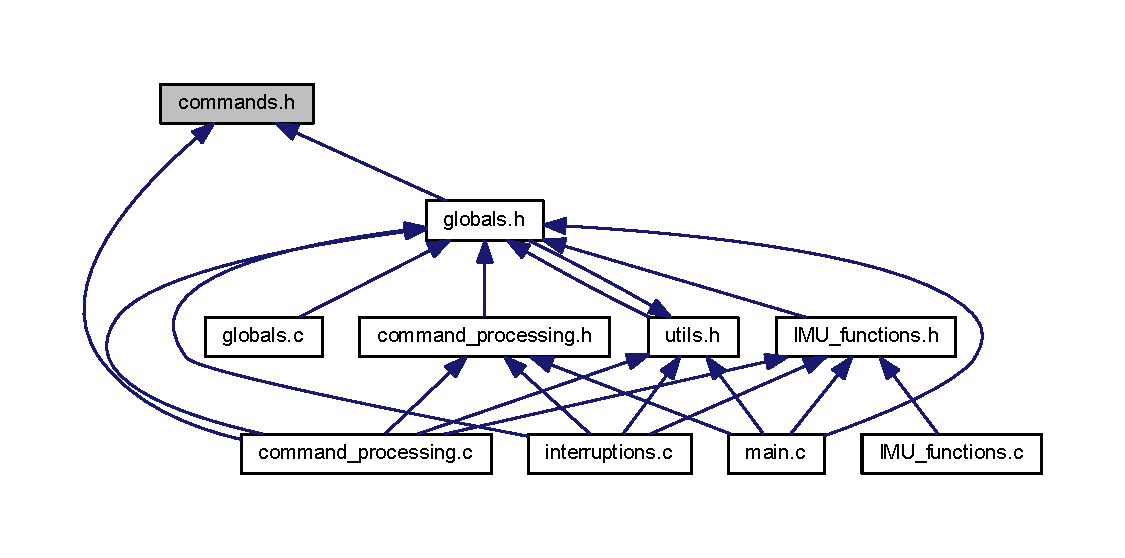
\includegraphics[width=350pt]{commands_8h__dep__incl}
\end{center}
\end{figure}
\subsection*{Macros}
\begin{DoxyCompactItemize}
\item 
\mbox{\label{commands_8h_ae3302107827a773be3200e459e7b24da}} 
\#define {\bfseries P\+A\+R\+A\+M\+\_\+\+B\+Y\+T\+E\+\_\+\+S\+L\+OT}~50
\item 
\mbox{\label{commands_8h_a3bab5133f6aa363d84307b39e17b0d74}} 
\#define {\bfseries P\+A\+R\+A\+M\+\_\+\+M\+E\+N\+U\+\_\+\+S\+L\+OT}~150
\end{DoxyCompactItemize}
\begin{Indent}\textbf{ QB Move Information Strings}\par
\begin{DoxyCompactItemize}
\item 
\mbox{\label{commands_8h_a2ba44fc5b8a316bd307d0baa9ab629ef}} 
\#define \textbf{ I\+N\+F\+O\+\_\+\+A\+LL}~0
\begin{DoxyCompactList}\small\item\em All system information. \end{DoxyCompactList}\item 
\mbox{\label{commands_8h_a1d08cadf994ec74db774800cfe81e499}} 
\#define \textbf{ I\+N\+F\+O\+\_\+\+R\+E\+A\+D\+I\+NG}~1
\begin{DoxyCompactList}\small\item\em I\+M\+Us reading information. \end{DoxyCompactList}\end{DoxyCompactItemize}
\end{Indent}
\subsection*{Enumerations}
\begin{DoxyCompactItemize}
\item 
\mbox{\label{commands_8h_a0eae1c82d20671c5d0b9b82b10070f1b}} 
enum {\bfseries acknowledgment\+\_\+values} \{ {\bfseries A\+C\+K\+\_\+\+E\+R\+R\+OR} = 0, 
{\bfseries A\+C\+K\+\_\+\+OK} = 1
 \}
\item 
\mbox{\label{commands_8h_aee7544e5fa6e2843ecdc3609602e56aa}} 
enum {\bfseries data\+\_\+types} \{ \newline
{\bfseries T\+Y\+P\+E\+\_\+\+F\+L\+AG} = 0, 
{\bfseries T\+Y\+P\+E\+\_\+\+I\+N\+T8} = 1, 
{\bfseries T\+Y\+P\+E\+\_\+\+U\+I\+N\+T8} = 2, 
{\bfseries T\+Y\+P\+E\+\_\+\+I\+N\+T16} = 3, 
\newline
{\bfseries T\+Y\+P\+E\+\_\+\+U\+I\+N\+T16} = 4, 
{\bfseries T\+Y\+P\+E\+\_\+\+I\+N\+T32} = 5, 
{\bfseries T\+Y\+P\+E\+\_\+\+U\+I\+N\+T32} = 6, 
{\bfseries T\+Y\+P\+E\+\_\+\+F\+L\+O\+AT} = 7, 
\newline
{\bfseries T\+Y\+P\+E\+\_\+\+D\+O\+U\+B\+LE} = 8
 \}
\end{DoxyCompactItemize}
\begin{Indent}\textbf{ QB Move Commands}\par
\begin{DoxyCompactItemize}
\item 
enum \textbf{ qbmove\+\_\+command} \{ \newline
\textbf{ C\+M\+D\+\_\+\+P\+I\+NG} = 0, 
\textbf{ C\+M\+D\+\_\+\+S\+T\+O\+R\+E\+\_\+\+P\+A\+R\+A\+MS} = 3, 
\textbf{ C\+M\+D\+\_\+\+S\+T\+O\+R\+E\+\_\+\+D\+E\+F\+A\+U\+L\+T\+\_\+\+P\+A\+R\+A\+MS} = 4, 
\textbf{ C\+M\+D\+\_\+\+R\+E\+S\+T\+O\+R\+E\+\_\+\+P\+A\+R\+A\+MS} = 5, 
\newline
\textbf{ C\+M\+D\+\_\+\+G\+E\+T\+\_\+\+I\+N\+FO} = 6, 
\textbf{ C\+M\+D\+\_\+\+S\+E\+T\+\_\+\+V\+A\+L\+UE} = 7, 
\textbf{ C\+M\+D\+\_\+\+G\+E\+T\+\_\+\+V\+A\+L\+UE} = 8, 
\textbf{ C\+M\+D\+\_\+\+B\+O\+O\+T\+L\+O\+A\+D\+ER} = 9, 
\newline
\textbf{ C\+M\+D\+\_\+\+I\+N\+I\+T\+\_\+\+M\+EM} = 10, 
\textbf{ C\+M\+D\+\_\+\+G\+E\+T\+\_\+\+P\+A\+R\+A\+M\+\_\+\+L\+I\+ST} = 12, 
\textbf{ C\+M\+D\+\_\+\+S\+E\+T\+\_\+\+B\+A\+U\+D\+R\+A\+TE} = 139, 
\textbf{ C\+M\+D\+\_\+\+G\+E\+T\+\_\+\+N\+\_\+\+I\+MU} = 160, 
\newline
{\bfseries C\+M\+D\+\_\+\+G\+E\+T\+\_\+\+I\+M\+U\+\_\+\+R\+E\+A\+D\+I\+N\+GS} = 161
 \}
\end{DoxyCompactItemize}
\end{Indent}


\subsection{Detailed Description}
Definitions for commands, parameters and packages. 

\begin{DoxyDate}{Date}
February 01, 2018 
\end{DoxyDate}
\begin{DoxyAuthor}{Author}
{\itshape Centro \char`\"{}\+E.\+Piaggio\char`\"{}} 
\end{DoxyAuthor}
\begin{DoxyCopyright}{Copyright}
(C) 2012-\/2016 qbrobotics. All rights reserved. 

(C) 2017-\/2018 Centro \char`\"{}\+E.\+Piaggio\char`\"{}. All rights reserved. 
\end{DoxyCopyright}


\subsection{Enumeration Type Documentation}
\mbox{\label{commands_8h_abf0494aabdc65d654a54044eddc9210b}} 
\index{commands.\+h@{commands.\+h}!qbmove\+\_\+command@{qbmove\+\_\+command}}
\index{qbmove\+\_\+command@{qbmove\+\_\+command}!commands.\+h@{commands.\+h}}
\subsubsection{qbmove\+\_\+command}
{\footnotesize\ttfamily enum \textbf{ qbmove\+\_\+command}}

\begin{DoxyEnumFields}{Enumerator}
\raisebox{\heightof{T}}[0pt][0pt]{\index{C\+M\+D\+\_\+\+P\+I\+NG@{C\+M\+D\+\_\+\+P\+I\+NG}!commands.\+h@{commands.\+h}}\index{commands.\+h@{commands.\+h}!C\+M\+D\+\_\+\+P\+I\+NG@{C\+M\+D\+\_\+\+P\+I\+NG}}}\mbox{\label{commands_8h_abf0494aabdc65d654a54044eddc9210ba1c0aa24c3612e77ea1a5ca1b82388da0}} 
C\+M\+D\+\_\+\+P\+I\+NG&Asks for a ping message. \\
\hline

\raisebox{\heightof{T}}[0pt][0pt]{\index{C\+M\+D\+\_\+\+S\+T\+O\+R\+E\+\_\+\+P\+A\+R\+A\+MS@{C\+M\+D\+\_\+\+S\+T\+O\+R\+E\+\_\+\+P\+A\+R\+A\+MS}!commands.\+h@{commands.\+h}}\index{commands.\+h@{commands.\+h}!C\+M\+D\+\_\+\+S\+T\+O\+R\+E\+\_\+\+P\+A\+R\+A\+MS@{C\+M\+D\+\_\+\+S\+T\+O\+R\+E\+\_\+\+P\+A\+R\+A\+MS}}}\mbox{\label{commands_8h_abf0494aabdc65d654a54044eddc9210bac7d1170961179d8dc5ec1b4aeb4f3116}} 
C\+M\+D\+\_\+\+S\+T\+O\+R\+E\+\_\+\+P\+A\+R\+A\+MS&Stores all parameters in memory and loads them \\
\hline

\raisebox{\heightof{T}}[0pt][0pt]{\index{C\+M\+D\+\_\+\+S\+T\+O\+R\+E\+\_\+\+D\+E\+F\+A\+U\+L\+T\+\_\+\+P\+A\+R\+A\+MS@{C\+M\+D\+\_\+\+S\+T\+O\+R\+E\+\_\+\+D\+E\+F\+A\+U\+L\+T\+\_\+\+P\+A\+R\+A\+MS}!commands.\+h@{commands.\+h}}\index{commands.\+h@{commands.\+h}!C\+M\+D\+\_\+\+S\+T\+O\+R\+E\+\_\+\+D\+E\+F\+A\+U\+L\+T\+\_\+\+P\+A\+R\+A\+MS@{C\+M\+D\+\_\+\+S\+T\+O\+R\+E\+\_\+\+D\+E\+F\+A\+U\+L\+T\+\_\+\+P\+A\+R\+A\+MS}}}\mbox{\label{commands_8h_abf0494aabdc65d654a54044eddc9210ba17d9c730cd01059737de14b9f062e44c}} 
C\+M\+D\+\_\+\+S\+T\+O\+R\+E\+\_\+\+D\+E\+F\+A\+U\+L\+T\+\_\+\+P\+A\+R\+A\+MS&Store current parameters as factory parameters. \\
\hline

\raisebox{\heightof{T}}[0pt][0pt]{\index{C\+M\+D\+\_\+\+R\+E\+S\+T\+O\+R\+E\+\_\+\+P\+A\+R\+A\+MS@{C\+M\+D\+\_\+\+R\+E\+S\+T\+O\+R\+E\+\_\+\+P\+A\+R\+A\+MS}!commands.\+h@{commands.\+h}}\index{commands.\+h@{commands.\+h}!C\+M\+D\+\_\+\+R\+E\+S\+T\+O\+R\+E\+\_\+\+P\+A\+R\+A\+MS@{C\+M\+D\+\_\+\+R\+E\+S\+T\+O\+R\+E\+\_\+\+P\+A\+R\+A\+MS}}}\mbox{\label{commands_8h_abf0494aabdc65d654a54044eddc9210ba7f13c143f54c74572776ffae219d33d7}} 
C\+M\+D\+\_\+\+R\+E\+S\+T\+O\+R\+E\+\_\+\+P\+A\+R\+A\+MS&Restore default factory parameters. \\
\hline

\raisebox{\heightof{T}}[0pt][0pt]{\index{C\+M\+D\+\_\+\+G\+E\+T\+\_\+\+I\+N\+FO@{C\+M\+D\+\_\+\+G\+E\+T\+\_\+\+I\+N\+FO}!commands.\+h@{commands.\+h}}\index{commands.\+h@{commands.\+h}!C\+M\+D\+\_\+\+G\+E\+T\+\_\+\+I\+N\+FO@{C\+M\+D\+\_\+\+G\+E\+T\+\_\+\+I\+N\+FO}}}\mbox{\label{commands_8h_abf0494aabdc65d654a54044eddc9210ba4681b714888632a2d8ad0a2140e4ba7f}} 
C\+M\+D\+\_\+\+G\+E\+T\+\_\+\+I\+N\+FO&Asks for a string of information about. \\
\hline

\raisebox{\heightof{T}}[0pt][0pt]{\index{C\+M\+D\+\_\+\+S\+E\+T\+\_\+\+V\+A\+L\+UE@{C\+M\+D\+\_\+\+S\+E\+T\+\_\+\+V\+A\+L\+UE}!commands.\+h@{commands.\+h}}\index{commands.\+h@{commands.\+h}!C\+M\+D\+\_\+\+S\+E\+T\+\_\+\+V\+A\+L\+UE@{C\+M\+D\+\_\+\+S\+E\+T\+\_\+\+V\+A\+L\+UE}}}\mbox{\label{commands_8h_abf0494aabdc65d654a54044eddc9210bac3ca8989b510cb78baff4425a0d47a67}} 
C\+M\+D\+\_\+\+S\+E\+T\+\_\+\+V\+A\+L\+UE&Not Used. \\
\hline

\raisebox{\heightof{T}}[0pt][0pt]{\index{C\+M\+D\+\_\+\+G\+E\+T\+\_\+\+V\+A\+L\+UE@{C\+M\+D\+\_\+\+G\+E\+T\+\_\+\+V\+A\+L\+UE}!commands.\+h@{commands.\+h}}\index{commands.\+h@{commands.\+h}!C\+M\+D\+\_\+\+G\+E\+T\+\_\+\+V\+A\+L\+UE@{C\+M\+D\+\_\+\+G\+E\+T\+\_\+\+V\+A\+L\+UE}}}\mbox{\label{commands_8h_abf0494aabdc65d654a54044eddc9210bac9a592ed746a114c7bfc0bd9d094263c}} 
C\+M\+D\+\_\+\+G\+E\+T\+\_\+\+V\+A\+L\+UE&Not Used. \\
\hline

\raisebox{\heightof{T}}[0pt][0pt]{\index{C\+M\+D\+\_\+\+B\+O\+O\+T\+L\+O\+A\+D\+ER@{C\+M\+D\+\_\+\+B\+O\+O\+T\+L\+O\+A\+D\+ER}!commands.\+h@{commands.\+h}}\index{commands.\+h@{commands.\+h}!C\+M\+D\+\_\+\+B\+O\+O\+T\+L\+O\+A\+D\+ER@{C\+M\+D\+\_\+\+B\+O\+O\+T\+L\+O\+A\+D\+ER}}}\mbox{\label{commands_8h_abf0494aabdc65d654a54044eddc9210bac72c6075e3464ea5abbe0c0d6e11559e}} 
C\+M\+D\+\_\+\+B\+O\+O\+T\+L\+O\+A\+D\+ER&Sets the bootloader modality to update the firmware \\
\hline

\raisebox{\heightof{T}}[0pt][0pt]{\index{C\+M\+D\+\_\+\+I\+N\+I\+T\+\_\+\+M\+EM@{C\+M\+D\+\_\+\+I\+N\+I\+T\+\_\+\+M\+EM}!commands.\+h@{commands.\+h}}\index{commands.\+h@{commands.\+h}!C\+M\+D\+\_\+\+I\+N\+I\+T\+\_\+\+M\+EM@{C\+M\+D\+\_\+\+I\+N\+I\+T\+\_\+\+M\+EM}}}\mbox{\label{commands_8h_abf0494aabdc65d654a54044eddc9210ba7bd24a7ad88af9a4e7c398a9ecb08ed4}} 
C\+M\+D\+\_\+\+I\+N\+I\+T\+\_\+\+M\+EM&Initialize the memory with the defalut values. \\
\hline

\raisebox{\heightof{T}}[0pt][0pt]{\index{C\+M\+D\+\_\+\+G\+E\+T\+\_\+\+P\+A\+R\+A\+M\+\_\+\+L\+I\+ST@{C\+M\+D\+\_\+\+G\+E\+T\+\_\+\+P\+A\+R\+A\+M\+\_\+\+L\+I\+ST}!commands.\+h@{commands.\+h}}\index{commands.\+h@{commands.\+h}!C\+M\+D\+\_\+\+G\+E\+T\+\_\+\+P\+A\+R\+A\+M\+\_\+\+L\+I\+ST@{C\+M\+D\+\_\+\+G\+E\+T\+\_\+\+P\+A\+R\+A\+M\+\_\+\+L\+I\+ST}}}\mbox{\label{commands_8h_abf0494aabdc65d654a54044eddc9210ba3e92a6e4c288be3abb6f3cfadf261e78}} 
C\+M\+D\+\_\+\+G\+E\+T\+\_\+\+P\+A\+R\+A\+M\+\_\+\+L\+I\+ST&Command to get the parameters list or to set a defined value chosen by the use \\
\hline

\raisebox{\heightof{T}}[0pt][0pt]{\index{C\+M\+D\+\_\+\+S\+E\+T\+\_\+\+B\+A\+U\+D\+R\+A\+TE@{C\+M\+D\+\_\+\+S\+E\+T\+\_\+\+B\+A\+U\+D\+R\+A\+TE}!commands.\+h@{commands.\+h}}\index{commands.\+h@{commands.\+h}!C\+M\+D\+\_\+\+S\+E\+T\+\_\+\+B\+A\+U\+D\+R\+A\+TE@{C\+M\+D\+\_\+\+S\+E\+T\+\_\+\+B\+A\+U\+D\+R\+A\+TE}}}\mbox{\label{commands_8h_abf0494aabdc65d654a54044eddc9210ba2ddc0e8c5f0a28ad470e881d1e196c47}} 
C\+M\+D\+\_\+\+S\+E\+T\+\_\+\+B\+A\+U\+D\+R\+A\+TE&Command for setting baudrate \\
\hline

\raisebox{\heightof{T}}[0pt][0pt]{\index{C\+M\+D\+\_\+\+G\+E\+T\+\_\+\+N\+\_\+\+I\+MU@{C\+M\+D\+\_\+\+G\+E\+T\+\_\+\+N\+\_\+\+I\+MU}!commands.\+h@{commands.\+h}}\index{commands.\+h@{commands.\+h}!C\+M\+D\+\_\+\+G\+E\+T\+\_\+\+N\+\_\+\+I\+MU@{C\+M\+D\+\_\+\+G\+E\+T\+\_\+\+N\+\_\+\+I\+MU}}}\mbox{\label{commands_8h_abf0494aabdc65d654a54044eddc9210ba7473c6bbdcfa7989ff1eeb5177aee530}} 
C\+M\+D\+\_\+\+G\+E\+T\+\_\+\+N\+\_\+\+I\+MU&of communication \\
\hline

\end{DoxyEnumFields}

\section{globals.\+c File Reference}
\label{globals_8c}\index{globals.\+c@{globals.\+c}}


Global variables.  


{\ttfamily \#include $<$globals.\+h$>$}\newline
Include dependency graph for globals.\+c\+:
\nopagebreak
\begin{figure}[H]
\begin{center}
\leavevmode
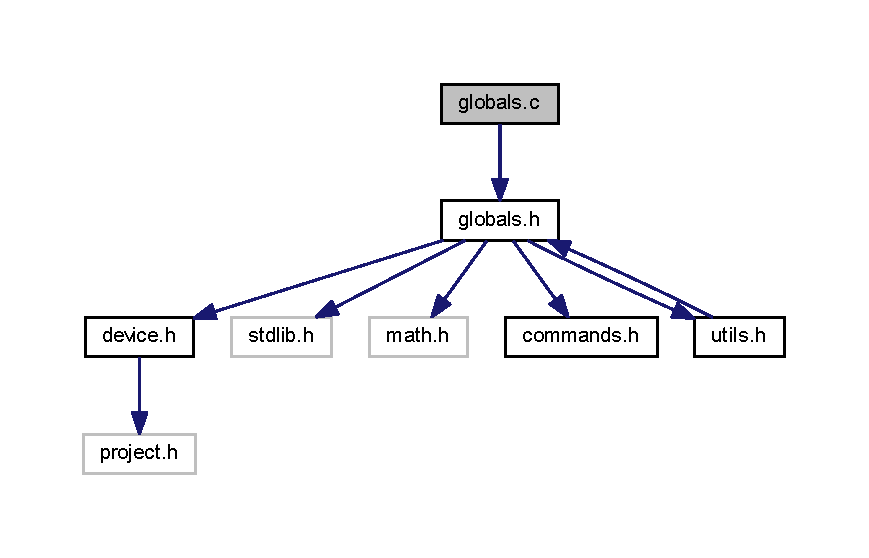
\includegraphics[width=350pt]{globals_8c__incl}
\end{center}
\end{figure}
\subsection*{Variables}
\begin{DoxyCompactItemize}
\item 
\mbox{\label{globals_8c_aa963ce8fafc11e104eb7ee22982d0345}} 
struct \textbf{ st\+\_\+data} {\bfseries g\+\_\+rx}
\item 
\mbox{\label{globals_8c_a44c3cbd8e234e0816f0334e29646a800}} 
struct \textbf{ st\+\_\+mem} g\+\_\+mem {\bfseries c\+\_\+mem}
\item 
\mbox{\label{globals_8c_ad47cd0e4d0fcf5739a88e52e949a8084}} 
uint32 {\bfseries timer\+\_\+value}
\item 
\mbox{\label{globals_8c_a9bab7f1b1cf2ba38d5968eee42644c32}} 
uint32 {\bfseries timer\+\_\+value0}
\item 
\mbox{\label{globals_8c_a1e6fda88dfdabc63859f8907eb702920}} 
C\+Y\+B\+IT {\bfseries interrupt\+\_\+flag}
\item 
\mbox{\label{globals_8c_a47118db87acd24ae6dac18b036f360ec}} 
uint8 {\bfseries N\+\_\+\+I\+M\+U\+\_\+\+Connected}
\item 
\mbox{\label{globals_8c_a99668f3210aba0be3baec19486621bce}} 
uint8 {\bfseries I\+M\+U\+\_\+connected} [N\+\_\+\+I\+M\+U\+\_\+\+M\+AX]
\item 
\mbox{\label{globals_8c_a86272fcfcab512d38a11824196df4bbc}} 
int {\bfseries imus\+\_\+data\+\_\+size}
\item 
\mbox{\label{globals_8c_aca96c483c3e269e3805aa861ced0aef5}} 
int {\bfseries single\+\_\+imu\+\_\+size} [N\+\_\+\+I\+M\+U\+\_\+\+M\+AX]
\item 
\mbox{\label{globals_8c_a86bb710944c248adeda63ded90db872a}} 
struct \textbf{ st\+\_\+imu} {\bfseries g\+\_\+imu} [N\+\_\+\+I\+M\+U\+\_\+\+M\+AX]
\item 
\mbox{\label{globals_8c_a9fa446daf1b4e3d6cc394fdc88e0ff63}} 
struct \textbf{ st\+\_\+imu} {\bfseries g\+\_\+imu\+New} [N\+\_\+\+I\+M\+U\+\_\+\+M\+AX]
\item 
\mbox{\label{globals_8c_a187c605f3898cf11e09f6f469c265920}} 
uint8 {\bfseries Accel} [N\+\_\+\+I\+M\+U\+\_\+\+M\+AX][6]
\item 
\mbox{\label{globals_8c_a49dba88a31d1b3b4190065b9ef1649fe}} 
uint8 {\bfseries Gyro} [N\+\_\+\+I\+M\+U\+\_\+\+M\+AX][6]
\item 
\mbox{\label{globals_8c_a5d88408ccb73729f049a52b4d1daaadf}} 
uint8 {\bfseries Mag} [N\+\_\+\+I\+M\+U\+\_\+\+M\+AX][6]
\item 
\mbox{\label{globals_8c_a1e598e1bdae5fe927fbd1f396161f3a6}} 
uint8 {\bfseries Mag\+Cal} [N\+\_\+\+I\+M\+U\+\_\+\+M\+AX][3]
\item 
\mbox{\label{globals_8c_af5f2d49e123a057d358297a34194ebdc}} 
uint8 {\bfseries Temp} [N\+\_\+\+I\+M\+U\+\_\+\+M\+AX][2]
\item 
\mbox{\label{globals_8c_ac0c4d3f055f976340a0e604e58b95a8a}} 
float {\bfseries Quat} [4] = \{1,0,0,0\}
\end{DoxyCompactItemize}


\subsection{Detailed Description}
Global variables. 

\begin{DoxyDate}{Date}
February 01, 2018 
\end{DoxyDate}
\begin{DoxyAuthor}{Author}
{\itshape Centro \char`\"{}\+E.\+Piaggio\char`\"{}} 
\end{DoxyAuthor}
\begin{DoxyCopyright}{Copyright}
(C) 2012-\/2016 qbrobotics. All rights reserved. 

(C) 2017-\/2018 Centro \char`\"{}\+E.\+Piaggio\char`\"{}. All rights reserved. 
\end{DoxyCopyright}

\section{globals.\+h File Reference}
\label{globals_8h}\index{globals.\+h@{globals.\+h}}


Global definitions and macros are set in this file.  


{\ttfamily \#include $<$device.\+h$>$}\newline
{\ttfamily \#include \char`\"{}stdlib.\+h\char`\"{}}\newline
{\ttfamily \#include \char`\"{}math.\+h\char`\"{}}\newline
{\ttfamily \#include \char`\"{}commands.\+h\char`\"{}}\newline
{\ttfamily \#include \char`\"{}utils.\+h\char`\"{}}\newline
Include dependency graph for globals.\+h\+:
\nopagebreak
\begin{figure}[H]
\begin{center}
\leavevmode
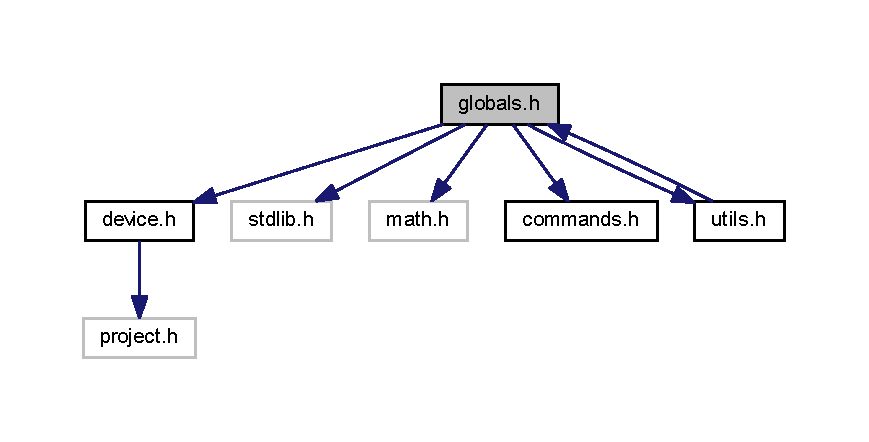
\includegraphics[width=350pt]{globals_8h__incl}
\end{center}
\end{figure}
This graph shows which files directly or indirectly include this file\+:
\nopagebreak
\begin{figure}[H]
\begin{center}
\leavevmode
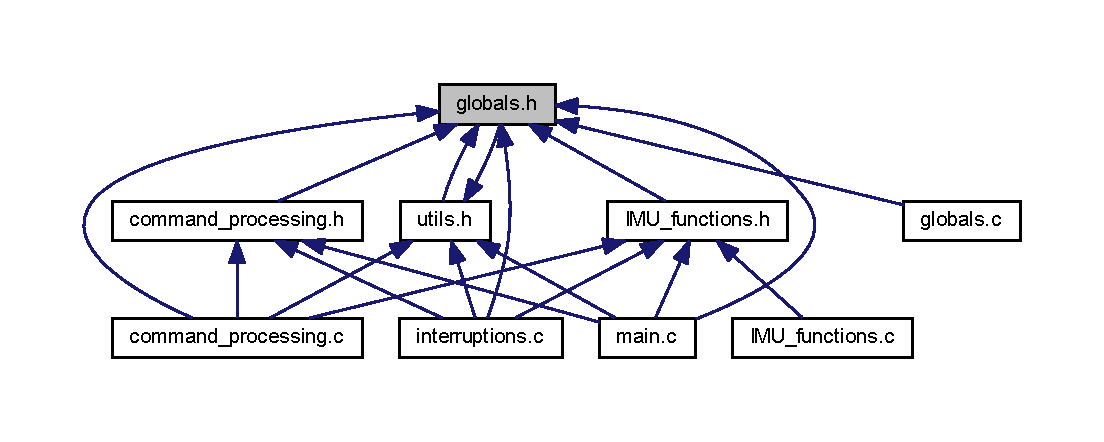
\includegraphics[width=350pt]{globals_8h__dep__incl}
\end{center}
\end{figure}
\subsection*{Data Structures}
\begin{DoxyCompactItemize}
\item 
struct \textbf{ st\+\_\+data}
\item 
struct \textbf{ st\+\_\+mem}
\item 
struct \textbf{ st\+\_\+imu}
\end{DoxyCompactItemize}
\subsection*{Macros}
\begin{DoxyCompactItemize}
\item 
\mbox{\label{globals_8h_a1c6d5de492ac61ad29aec7aa9a436bbf}} 
\#define {\bfseries V\+E\+R\+S\+I\+ON}~\char`\"{}I\+M\+Uboard v 1.\+1\char`\"{}
\item 
\mbox{\label{globals_8h_a8e4d7a571850d3268c9b780b171474e6}} 
\#define {\bfseries N\+\_\+\+I\+M\+U\+\_\+\+M\+AX}~17
\item 
\mbox{\label{globals_8h_a160df9a8c910183dfc855b2e6746f6a3}} 
\#define {\bfseries N\+U\+M\+\_\+\+O\+F\+\_\+\+D\+A\+TA}~5
\item 
\mbox{\label{globals_8h_a80db2dce057c92400a7fb1678bc0b0a8}} 
\#define {\bfseries C\+A\+L\+I\+B\+R\+A\+T\+I\+O\+N\+\_\+\+D\+IV}~10
\item 
\mbox{\label{globals_8h_a14df76a41da04070ee775565e8d67e81}} 
\#define {\bfseries D\+I\+V\+\_\+\+I\+N\+I\+T\+\_\+\+V\+A\+L\+UE}~1
\item 
\mbox{\label{globals_8h_abf6c9afec04b86961e177e0646401ace}} 
\#define {\bfseries D\+M\+A\+\_\+\+B\+Y\+T\+E\+S\+\_\+\+P\+E\+R\+\_\+\+B\+U\+R\+ST}~2
\item 
\mbox{\label{globals_8h_ab4613f8bee68bc68fa6fe94a3ae6d568}} 
\#define {\bfseries D\+M\+A\+\_\+\+R\+E\+Q\+U\+E\+S\+T\+\_\+\+P\+E\+R\+\_\+\+B\+U\+R\+ST}~1
\item 
\mbox{\label{globals_8h_a3cc2eedb40809a1f15ad841c8abbcebf}} 
\#define {\bfseries D\+M\+A\+\_\+\+S\+R\+C\+\_\+\+B\+A\+SE}~(C\+Y\+D\+E\+V\+\_\+\+P\+E\+R\+I\+P\+H\+\_\+\+B\+A\+SE)
\item 
\mbox{\label{globals_8h_aa54e301f446a66cbf8c943d920c8e967}} 
\#define {\bfseries D\+M\+A\+\_\+\+D\+S\+T\+\_\+\+B\+A\+SE}~(C\+Y\+D\+E\+V\+\_\+\+S\+R\+A\+M\+\_\+\+B\+A\+SE)
\item 
\mbox{\label{globals_8h_aea55597952638136c7c929b238904c82}} 
\#define {\bfseries W\+A\+I\+T\+\_\+\+S\+T\+A\+RT}~0
\item 
\mbox{\label{globals_8h_a6a6a0bb02e515a094c3e7ea1bcb66fcc}} 
\#define {\bfseries W\+A\+I\+T\+\_\+\+ID}~1
\item 
\mbox{\label{globals_8h_a235d2d0eac7e9af190ebafb84df37fd9}} 
\#define {\bfseries W\+A\+I\+T\+\_\+\+L\+E\+N\+G\+TH}~2
\item 
\mbox{\label{globals_8h_a3b4d8a5e259fa47a909adefcda3bfb80}} 
\#define {\bfseries R\+E\+C\+E\+I\+VE}~3
\item 
\mbox{\label{globals_8h_abf4aedd34d31b63b63061c975d872580}} 
\#define {\bfseries U\+N\+L\+O\+AD}~4
\item 
\mbox{\label{globals_8h_a42c6406a75a89d50c9f1b9c86388565c}} 
\#define {\bfseries S\+P\+I\+\_\+\+D\+E\+L\+A\+Y\+\_\+\+L\+OW}~10
\item 
\mbox{\label{globals_8h_a054002df34537a2a4ff6f520b65f1ba4}} 
\#define {\bfseries S\+P\+I\+\_\+\+D\+E\+L\+A\+Y\+\_\+\+H\+I\+GH}~100
\item 
\mbox{\label{globals_8h_aa93f0eb578d23995850d61f7d61c55c1}} 
\#define {\bfseries F\+A\+L\+SE}~0
\item 
\mbox{\label{globals_8h_aa8cecfc5c5c054d2875c03e77b7be15d}} 
\#define {\bfseries T\+R\+UE}~1
\item 
\mbox{\label{globals_8h_a0f5a7e2ead9cd507bf8fc9a6f785f012}} 
\#define {\bfseries D\+E\+F\+A\+U\+L\+T\+\_\+\+E\+E\+P\+R\+O\+M\+\_\+\+D\+I\+S\+P\+L\+A\+C\+E\+M\+E\+NT}~8
\end{DoxyCompactItemize}
\subsection*{Variables}
\begin{DoxyCompactItemize}
\item 
\mbox{\label{globals_8h_aa963ce8fafc11e104eb7ee22982d0345}} 
struct \textbf{ st\+\_\+data} {\bfseries g\+\_\+rx}
\item 
\mbox{\label{globals_8h_a44c3cbd8e234e0816f0334e29646a800}} 
struct \textbf{ st\+\_\+mem} g\+\_\+mem {\bfseries c\+\_\+mem}
\item 
\mbox{\label{globals_8h_ad47cd0e4d0fcf5739a88e52e949a8084}} 
uint32 {\bfseries timer\+\_\+value}
\item 
\mbox{\label{globals_8h_a9bab7f1b1cf2ba38d5968eee42644c32}} 
uint32 {\bfseries timer\+\_\+value0}
\item 
\mbox{\label{globals_8h_a1e6fda88dfdabc63859f8907eb702920}} 
C\+Y\+B\+IT {\bfseries interrupt\+\_\+flag}
\item 
\mbox{\label{globals_8h_a47118db87acd24ae6dac18b036f360ec}} 
uint8 {\bfseries N\+\_\+\+I\+M\+U\+\_\+\+Connected}
\item 
\mbox{\label{globals_8h_a99668f3210aba0be3baec19486621bce}} 
uint8 {\bfseries I\+M\+U\+\_\+connected} [N\+\_\+\+I\+M\+U\+\_\+\+M\+AX]
\item 
\mbox{\label{globals_8h_a86272fcfcab512d38a11824196df4bbc}} 
int {\bfseries imus\+\_\+data\+\_\+size}
\item 
\mbox{\label{globals_8h_aca96c483c3e269e3805aa861ced0aef5}} 
int {\bfseries single\+\_\+imu\+\_\+size} [N\+\_\+\+I\+M\+U\+\_\+\+M\+AX]
\item 
\mbox{\label{globals_8h_a86bb710944c248adeda63ded90db872a}} 
struct \textbf{ st\+\_\+imu} {\bfseries g\+\_\+imu} [N\+\_\+\+I\+M\+U\+\_\+\+M\+AX]
\item 
\mbox{\label{globals_8h_a9fa446daf1b4e3d6cc394fdc88e0ff63}} 
struct \textbf{ st\+\_\+imu} {\bfseries g\+\_\+imu\+New} [N\+\_\+\+I\+M\+U\+\_\+\+M\+AX]
\item 
\mbox{\label{globals_8h_a187c605f3898cf11e09f6f469c265920}} 
uint8 {\bfseries Accel} [N\+\_\+\+I\+M\+U\+\_\+\+M\+AX][6]
\item 
\mbox{\label{globals_8h_a49dba88a31d1b3b4190065b9ef1649fe}} 
uint8 {\bfseries Gyro} [N\+\_\+\+I\+M\+U\+\_\+\+M\+AX][6]
\item 
\mbox{\label{globals_8h_a5d88408ccb73729f049a52b4d1daaadf}} 
uint8 {\bfseries Mag} [N\+\_\+\+I\+M\+U\+\_\+\+M\+AX][6]
\item 
\mbox{\label{globals_8h_a1e598e1bdae5fe927fbd1f396161f3a6}} 
uint8 {\bfseries Mag\+Cal} [N\+\_\+\+I\+M\+U\+\_\+\+M\+AX][3]
\item 
\mbox{\label{globals_8h_af5f2d49e123a057d358297a34194ebdc}} 
uint8 {\bfseries Temp} [N\+\_\+\+I\+M\+U\+\_\+\+M\+AX][2]
\item 
\mbox{\label{globals_8h_ac0c4d3f055f976340a0e604e58b95a8a}} 
float {\bfseries Quat} [4]
\end{DoxyCompactItemize}


\subsection{Detailed Description}
Global definitions and macros are set in this file. 

\begin{DoxyDate}{Date}
February 01, 2018 
\end{DoxyDate}
\begin{DoxyAuthor}{Author}
{\itshape Centro \char`\"{}\+E.\+Piaggio\char`\"{}} 
\end{DoxyAuthor}
\begin{DoxyCopyright}{Copyright}
(C) 2012-\/2016 qbrobotics. All rights reserved. 

(C) 2017-\/2018 Centro \char`\"{}\+E.\+Piaggio\char`\"{}. All rights reserved. 
\end{DoxyCopyright}

\section{I\+M\+U\+\_\+functions.\+c File Reference}
\label{_i_m_u__functions_8c}\index{I\+M\+U\+\_\+functions.\+c@{I\+M\+U\+\_\+functions.\+c}}


Implementation of I\+MU module functions.  


{\ttfamily \#include $<$I\+M\+U\+\_\+functions.\+h$>$}\newline
{\ttfamily \#include $<$S\+P\+I\+\_\+\+I\+M\+U.\+h$>$}\newline
Include dependency graph for I\+M\+U\+\_\+functions.\+c\+:
\nopagebreak
\begin{figure}[H]
\begin{center}
\leavevmode
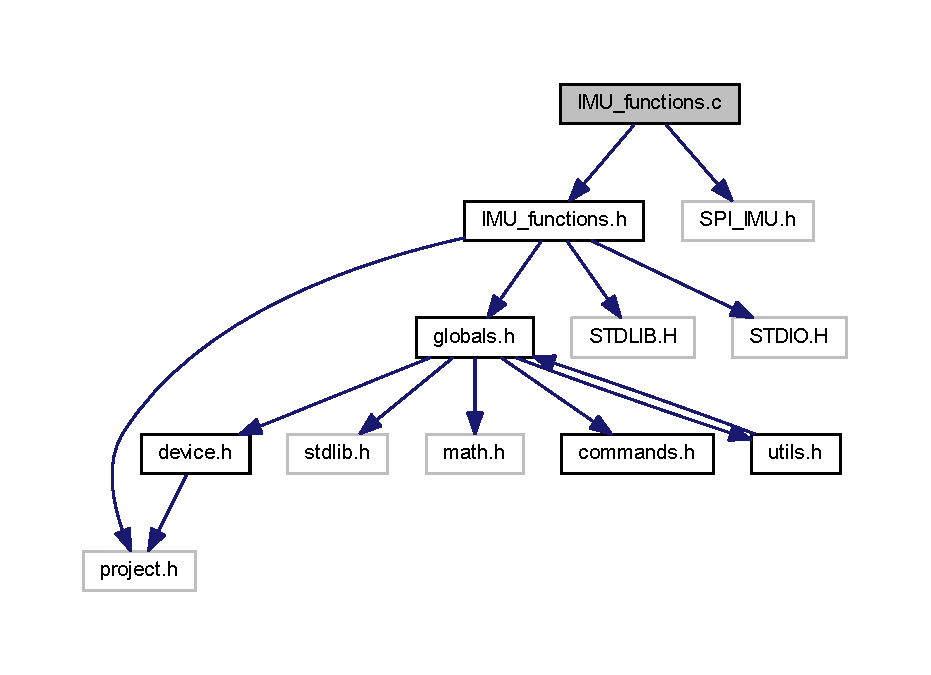
\includegraphics[width=350pt]{_i_m_u__functions_8c__incl}
\end{center}
\end{figure}
\subsection*{Functions}
\begin{DoxyCompactItemize}
\item 
\mbox{\label{_i_m_u__functions_8c_a950a5a57e4188823c580d054ed2db16a}} 
void {\bfseries Imus\+Reset} ()
\item 
\mbox{\label{_i_m_u__functions_8c_ac4f81f61837e6a132dfceb5bb93b06fa}} 
void {\bfseries Init\+I\+MU} ()
\item 
\mbox{\label{_i_m_u__functions_8c_ac95975151b543b5265bc1e470aabf465}} 
void {\bfseries Init\+I\+M\+U\+Mag\+Cal} ()
\item 
\mbox{\label{_i_m_u__functions_8c_a3bb201c102e53b1b56398272fa105fbb}} 
void {\bfseries Chip\+Selector} (int n)
\item 
\mbox{\label{_i_m_u__functions_8c_a83f0630cb5ff556322c8cf56b6c6afc0}} 
void {\bfseries Init\+I\+M\+Ugeneral} ()
\item 
\mbox{\label{_i_m_u__functions_8c_a45df9ddb73de250cebfa02bf1d72bd97}} 
void {\bfseries Read\+I\+MU} (int n)
\item 
\mbox{\label{_i_m_u__functions_8c_a0290185f5b71ddb96ea13ce0a1ff48e7}} 
void {\bfseries Read\+Acc} (int n)
\item 
\mbox{\label{_i_m_u__functions_8c_ab8ae2a28912ce4a548b3603e86b22ae9}} 
void {\bfseries Read\+Gyro} (int n)
\item 
\mbox{\label{_i_m_u__functions_8c_a2ee29250f51422fa3d76df77335cce26}} 
void {\bfseries Read\+Mag} (int n)
\item 
\mbox{\label{_i_m_u__functions_8c_aad3b4856a76c623025484fe5b931bdd4}} 
void {\bfseries Read\+Mag\+Cal} (int n)
\item 
\mbox{\label{_i_m_u__functions_8c_a8eeecefb2efe7e01711fb9448c31ae76}} 
void {\bfseries Read\+Quat} (int n)
\item 
\mbox{\label{_i_m_u__functions_8c_a27bf3026dfe4cb0d6d255decc9944d71}} 
void {\bfseries Read\+All\+I\+M\+Us} ()
\item 
\mbox{\label{_i_m_u__functions_8c_ab0883cd12ebf2937fd6da478ac3ab976}} 
void {\bfseries Read\+Temp} (int n)
\item 
\mbox{\label{_i_m_u__functions_8c_af429837786eebd63058e26b3c86ac17a}} 
void {\bfseries Write\+Control\+Register} (uint8 address, uint8 dta)
\item 
\mbox{\label{_i_m_u__functions_8c_a209b21711f8765bb41e1823aab7b995b}} 
uint8 {\bfseries Read\+Control\+Register} (uint8 address)
\item 
\mbox{\label{_i_m_u__functions_8c_a26f85d9c393e73879461861d2ac87379}} 
void {\bfseries S\+P\+I\+\_\+delay} ()
\end{DoxyCompactItemize}
\subsection*{Variables}
\begin{DoxyCompactItemize}
\item 
\mbox{\label{_i_m_u__functions_8c_a187c605f3898cf11e09f6f469c265920}} 
uint8 {\bfseries Accel} [N\+\_\+\+I\+M\+U\+\_\+\+M\+AX][6]
\item 
\mbox{\label{_i_m_u__functions_8c_a49dba88a31d1b3b4190065b9ef1649fe}} 
uint8 {\bfseries Gyro} [N\+\_\+\+I\+M\+U\+\_\+\+M\+AX][6]
\item 
\mbox{\label{_i_m_u__functions_8c_a5d88408ccb73729f049a52b4d1daaadf}} 
uint8 {\bfseries Mag} [N\+\_\+\+I\+M\+U\+\_\+\+M\+AX][6]
\item 
\mbox{\label{_i_m_u__functions_8c_a1e598e1bdae5fe927fbd1f396161f3a6}} 
uint8 {\bfseries Mag\+Cal} [N\+\_\+\+I\+M\+U\+\_\+\+M\+AX][3]
\end{DoxyCompactItemize}


\subsection{Detailed Description}
Implementation of I\+MU module functions. 

\begin{DoxyDate}{Date}
February 01, 2018 
\end{DoxyDate}
\begin{DoxyAuthor}{Author}
{\itshape Centro \char`\"{}\+E.\+Piaggio\char`\"{}} 
\end{DoxyAuthor}
\begin{DoxyCopyright}{Copyright}
(C) 2012-\/2016 qbrobotics. All rights reserved. 

(C) 2017-\/2018 Centro \char`\"{}\+E.\+Piaggio\char`\"{}. All rights reserved. 
\end{DoxyCopyright}

\section{I\+M\+U\+\_\+functions.\+h File Reference}
\label{_i_m_u__functions_8h}\index{I\+M\+U\+\_\+functions.\+h@{I\+M\+U\+\_\+functions.\+h}}


Definition of I\+MU module functions.  


{\ttfamily \#include $<$project.\+h$>$}\newline
{\ttfamily \#include $<$globals.\+h$>$}\newline
{\ttfamily \#include $<$S\+T\+D\+L\+I\+B.\+H$>$}\newline
{\ttfamily \#include $<$S\+T\+D\+I\+O.\+H$>$}\newline
Include dependency graph for I\+M\+U\+\_\+functions.\+h\+:
\nopagebreak
\begin{figure}[H]
\begin{center}
\leavevmode
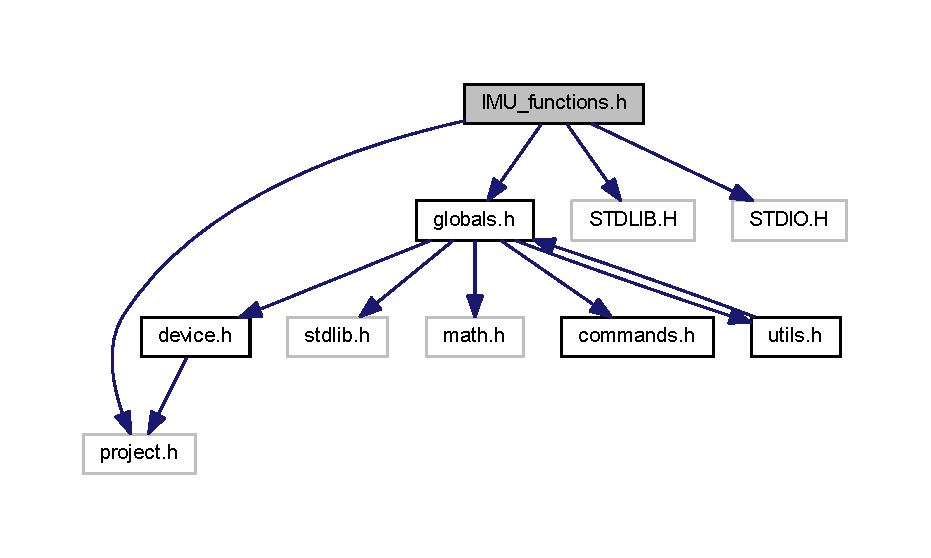
\includegraphics[width=350pt]{_i_m_u__functions_8h__incl}
\end{center}
\end{figure}
This graph shows which files directly or indirectly include this file\+:
\nopagebreak
\begin{figure}[H]
\begin{center}
\leavevmode
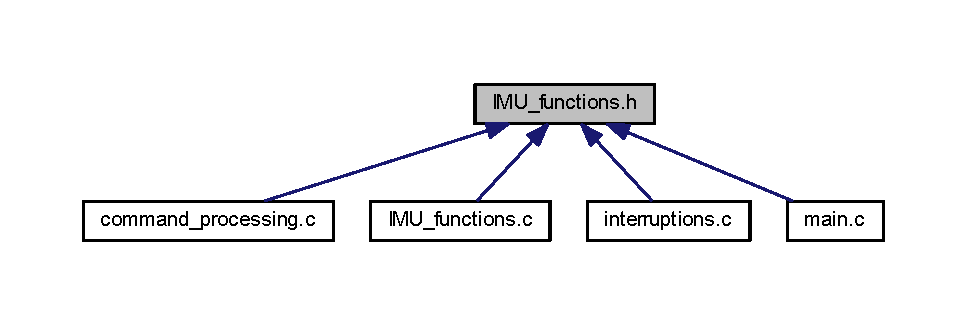
\includegraphics[width=350pt]{_i_m_u__functions_8h__dep__incl}
\end{center}
\end{figure}
\subsection*{Macros}
\begin{DoxyCompactItemize}
\item 
\mbox{\label{_i_m_u__functions_8h_a8f10e1abef86f90469efde459cc8e38a}} 
\#define {\bfseries M\+P\+U9250\+\_\+\+R\+CR}~0x80
\item 
\mbox{\label{_i_m_u__functions_8h_a04b6efd4a598a844bb53ed54aa34eca9}} 
\#define {\bfseries M\+P\+U9250\+\_\+\+W\+CR}~0x00
\item 
\mbox{\label{_i_m_u__functions_8h_a20204154f2c4969a76a4cfb351f092bd}} 
\#define {\bfseries M\+P\+U9250\+\_\+\+C\+O\+N\+F\+IG}~0x1A
\item 
\mbox{\label{_i_m_u__functions_8h_a8573879ec5b32b8e398fca47a6af8730}} 
\#define {\bfseries M\+P\+U9250\+\_\+\+G\+Y\+R\+O\+\_\+\+C\+O\+N\+F\+IG}~0x1B
\item 
\mbox{\label{_i_m_u__functions_8h_a98d764ea0ee5c3e4295ce7d1159d1b8f}} 
\#define {\bfseries M\+P\+U9250\+\_\+\+A\+C\+C\+E\+L\+\_\+\+C\+O\+N\+F\+IG}~0x1C
\item 
\mbox{\label{_i_m_u__functions_8h_af6cd76f367486f0c1c1a332d7969a80c}} 
\#define {\bfseries M\+P\+U9250\+\_\+\+A\+C\+C\+E\+L\+\_\+\+C\+O\+N\+F\+I\+G2}~0x1D
\item 
\mbox{\label{_i_m_u__functions_8h_a233902a190292b4092ed81dde3d9c741}} 
\#define {\bfseries M\+P\+U9250\+\_\+\+A\+C\+C\+E\+L\+\_\+\+X\+O\+U\+T\+\_\+H}~0x3B
\item 
\mbox{\label{_i_m_u__functions_8h_a68555dd7b566c506a3a903deba714188}} 
\#define {\bfseries M\+P\+U9250\+\_\+\+A\+C\+C\+E\+L\+\_\+\+X\+O\+U\+T\+\_\+L}~0x3C
\item 
\mbox{\label{_i_m_u__functions_8h_a74535eaadba66549faa09ba31a31f4b4}} 
\#define {\bfseries M\+P\+U9250\+\_\+\+A\+C\+C\+E\+L\+\_\+\+Y\+O\+U\+T\+\_\+H}~0x3D
\item 
\mbox{\label{_i_m_u__functions_8h_ad5d5e68cf15657c7ed9ec259a8cbcd81}} 
\#define {\bfseries M\+P\+U9250\+\_\+\+A\+C\+C\+E\+L\+\_\+\+Y\+O\+U\+T\+\_\+L}~0x3E
\item 
\mbox{\label{_i_m_u__functions_8h_ac112304e8cbba1dc9ccaa99773adf9cd}} 
\#define {\bfseries M\+P\+U9250\+\_\+\+A\+C\+C\+E\+L\+\_\+\+Z\+O\+U\+T\+\_\+H}~0x3F
\item 
\mbox{\label{_i_m_u__functions_8h_a964d6c7c4744ef0c32c22038f7025c05}} 
\#define {\bfseries M\+P\+U9250\+\_\+\+A\+C\+C\+E\+L\+\_\+\+Z\+O\+U\+T\+\_\+L}~0x40
\item 
\mbox{\label{_i_m_u__functions_8h_afa30ca80a7c6bb0a8249fa8d6dd95a0f}} 
\#define {\bfseries M\+P\+U9250\+\_\+\+T\+E\+M\+P\+\_\+\+O\+U\+T\+\_\+H}~0x41
\item 
\mbox{\label{_i_m_u__functions_8h_af95af2d67b983b2b3b814df7fe76233c}} 
\#define {\bfseries M\+P\+U9250\+\_\+\+T\+E\+M\+P\+\_\+\+O\+U\+T\+\_\+L}~0x42
\item 
\mbox{\label{_i_m_u__functions_8h_acaa2d67e1c58af7d682dc492acb8a911}} 
\#define {\bfseries M\+P\+U9250\+\_\+\+G\+Y\+R\+O\+\_\+\+X\+O\+U\+T\+\_\+H}~0x43
\item 
\mbox{\label{_i_m_u__functions_8h_acabd4ef05dfc9b0322a2b7353adadbb7}} 
\#define {\bfseries M\+P\+U9250\+\_\+\+G\+Y\+R\+O\+\_\+\+X\+O\+U\+T\+\_\+L}~0x44
\item 
\mbox{\label{_i_m_u__functions_8h_aacdf26a239b0cd31d9d7bc9ba812f94f}} 
\#define {\bfseries M\+P\+U9250\+\_\+\+G\+Y\+R\+O\+\_\+\+Y\+O\+U\+T\+\_\+H}~0x45
\item 
\mbox{\label{_i_m_u__functions_8h_a2fa6a36ab2a3e9a0887a66f00083313a}} 
\#define {\bfseries M\+P\+U9250\+\_\+\+G\+Y\+R\+O\+\_\+\+Y\+O\+U\+T\+\_\+L}~0x46
\item 
\mbox{\label{_i_m_u__functions_8h_a167d6cef38aada435a7926b3ed9faa58}} 
\#define {\bfseries M\+P\+U9250\+\_\+\+G\+Y\+R\+O\+\_\+\+Z\+O\+U\+T\+\_\+H}~0x47
\item 
\mbox{\label{_i_m_u__functions_8h_a49bf44f22ff73221ef1f12da1b418a4c}} 
\#define {\bfseries M\+P\+U9250\+\_\+\+G\+Y\+R\+O\+\_\+\+Z\+O\+U\+T\+\_\+L}~0x48
\item 
\mbox{\label{_i_m_u__functions_8h_ac99d5d7a6fe9478e88b905e871fc03fd}} 
\#define {\bfseries M\+P\+U9250\+\_\+\+U\+S\+E\+R\+\_\+\+C\+T\+RL}~0x6A
\item 
\mbox{\label{_i_m_u__functions_8h_a2a9d837bb715d6c7ba3c14a4fa5433a0}} 
\#define {\bfseries M\+P\+U9250\+\_\+\+P\+W\+R\+\_\+\+M\+G\+M\+T\+\_\+1}~0x6B
\item 
\mbox{\label{_i_m_u__functions_8h_abbeb9762be6f9443df3c57561c8c3985}} 
\#define {\bfseries M\+P\+U9250\+\_\+\+W\+H\+O\+\_\+\+A\+M\+\_\+I}~0x75
\item 
\mbox{\label{_i_m_u__functions_8h_a9cb58e6b0474117ba9d0db2ae7c39641}} 
\#define {\bfseries M\+P\+U9250\+\_\+\+F\+I\+F\+O\+\_\+\+EN}~0x23
\item 
\mbox{\label{_i_m_u__functions_8h_aa384279b17d3d7d9ffea2c5ada427c5b}} 
\#define {\bfseries M\+P\+U9250\+\_\+\+I2\+C\+\_\+\+M\+S\+T\+\_\+\+C\+T\+RL}~0x24
\item 
\mbox{\label{_i_m_u__functions_8h_a23f87cacaa22c223b357f3bfc4feed28}} 
\#define {\bfseries M\+P\+U9250\+\_\+\+I2\+C\+\_\+\+S\+L\+V0\+\_\+\+A\+D\+DR}~0x25
\item 
\mbox{\label{_i_m_u__functions_8h_ad5819386ba91b6b113ff8cf8335e0679}} 
\#define {\bfseries M\+P\+U9250\+\_\+\+I2\+C\+\_\+\+S\+L\+V0\+\_\+\+R\+EG}~0x26
\item 
\mbox{\label{_i_m_u__functions_8h_a1513e5f1f2c5ca628f67d212ab4f5f12}} 
\#define {\bfseries M\+P\+U9250\+\_\+\+I2\+C\+\_\+\+S\+L\+V0\+\_\+\+C\+T\+RL}~0x27
\item 
\mbox{\label{_i_m_u__functions_8h_a4c75a33c83923d516cb845ca8ca0d3dc}} 
\#define {\bfseries M\+P\+U9250\+\_\+\+I2\+C\+\_\+\+S\+L\+V1\+\_\+\+A\+D\+DR}~0x28
\item 
\mbox{\label{_i_m_u__functions_8h_ade10530b44c603a3a1c133cbb407c3c0}} 
\#define {\bfseries M\+P\+U9250\+\_\+\+I2\+C\+\_\+\+S\+L\+V1\+\_\+\+R\+EG}~0x29
\item 
\mbox{\label{_i_m_u__functions_8h_aae60d3360aeba41250cfe5db3aa19ea1}} 
\#define {\bfseries M\+P\+U9250\+\_\+\+I2\+C\+\_\+\+S\+L\+V1\+\_\+\+C\+T\+RL}~0x2A
\item 
\mbox{\label{_i_m_u__functions_8h_a89ebc64bc3c3659eb1a8faeb53f2f1ef}} 
\#define {\bfseries M\+P\+U9250\+\_\+\+E\+X\+T\+\_\+\+S\+E\+N\+S\+\_\+\+D\+A\+T\+A\+\_\+00}~0x49
\item 
\mbox{\label{_i_m_u__functions_8h_a5f7838ce33b1da366466972b3230e39c}} 
\#define {\bfseries M\+P\+U9250\+\_\+\+E\+X\+T\+\_\+\+S\+E\+N\+S\+\_\+\+D\+A\+T\+A\+\_\+01}~0x4A
\item 
\mbox{\label{_i_m_u__functions_8h_aebddf028777b182e7281a6257058d242}} 
\#define {\bfseries M\+P\+U9250\+\_\+\+E\+X\+T\+\_\+\+S\+E\+N\+S\+\_\+\+D\+A\+T\+A\+\_\+02}~0x4B
\item 
\mbox{\label{_i_m_u__functions_8h_a5d3058dc98d943b9ac16259e6f5f5c56}} 
\#define {\bfseries M\+P\+U9250\+\_\+\+E\+X\+T\+\_\+\+S\+E\+N\+S\+\_\+\+D\+A\+T\+A\+\_\+03}~0x4C
\item 
\mbox{\label{_i_m_u__functions_8h_a6456046467c05d4148dc4129d7d98ab2}} 
\#define {\bfseries M\+P\+U9250\+\_\+\+E\+X\+T\+\_\+\+S\+E\+N\+S\+\_\+\+D\+A\+T\+A\+\_\+04}~0x4D
\item 
\mbox{\label{_i_m_u__functions_8h_a4bfcbc345ce09aaa3a8ba17423ae35c6}} 
\#define {\bfseries M\+P\+U9250\+\_\+\+E\+X\+T\+\_\+\+S\+E\+N\+S\+\_\+\+D\+A\+T\+A\+\_\+05}~0x4E
\item 
\mbox{\label{_i_m_u__functions_8h_ae45a312a0d42f4c1192e1eb999aa6421}} 
\#define {\bfseries M\+P\+U9250\+\_\+\+E\+X\+T\+\_\+\+S\+E\+N\+S\+\_\+\+D\+A\+T\+A\+\_\+06}~0x4F
\item 
\mbox{\label{_i_m_u__functions_8h_a971c0b1d68d1a29a0508d50cfbf1e228}} 
\#define {\bfseries M\+P\+U9250\+\_\+\+E\+X\+T\+\_\+\+S\+E\+N\+S\+\_\+\+D\+A\+T\+A\+\_\+07}~0x50
\item 
\mbox{\label{_i_m_u__functions_8h_a42180ecf00b8b7f23c4649f0c440e842}} 
\#define {\bfseries M\+P\+U9250\+\_\+\+I2\+C\+\_\+\+S\+L\+V0\+\_\+\+D0}~0x63
\item 
\mbox{\label{_i_m_u__functions_8h_a39ba244fbbbe56cce3b39bb05852aa6a}} 
\#define {\bfseries M\+P\+U9250\+\_\+\+I2\+C\+\_\+\+S\+L\+V1\+\_\+\+D0}~0x64
\item 
\mbox{\label{_i_m_u__functions_8h_a3dd3301a852bb70ba5038cf0cb75f9d5}} 
\#define {\bfseries M\+P\+U9250\+\_\+\+I2\+C\+\_\+\+M\+S\+T\+\_\+\+D\+E\+L\+A\+Y\+\_\+\+C\+T\+RL}~0x67
\item 
\mbox{\label{_i_m_u__functions_8h_a7aa2f4bed039afe22d25a3c023a6e460}} 
\#define {\bfseries A\+K8936\+\_\+\+A\+D\+D\+R\+E\+SS}~0x0C
\item 
\mbox{\label{_i_m_u__functions_8h_a1af6a72066d440cb29d4ca2afecfb0c2}} 
\#define {\bfseries A\+K8936\+\_\+\+W\+IA}~0x00
\item 
\mbox{\label{_i_m_u__functions_8h_a22efa59adef08d5b45ff078de5345ccc}} 
\#define {\bfseries A\+K8936\+\_\+\+I\+N\+FO}~0x01
\item 
\mbox{\label{_i_m_u__functions_8h_ad19fd876dda2a0eeb1ca5520479e7efd}} 
\#define {\bfseries A\+K8936\+\_\+\+S\+T1}~0x02
\item 
\mbox{\label{_i_m_u__functions_8h_a5b25454e155a7df7aafffd99cd3c0211}} 
\#define {\bfseries A\+K8936\+\_\+\+X\+O\+U\+T\+\_\+L}~0x03
\item 
\mbox{\label{_i_m_u__functions_8h_a2cac47374e87bbe185a28f1bea0dae3a}} 
\#define {\bfseries A\+K8936\+\_\+\+X\+O\+U\+T\+\_\+H}~0x04
\item 
\mbox{\label{_i_m_u__functions_8h_a7ff211c31fa6aae15e88f2ea72c8d3ea}} 
\#define {\bfseries A\+K8936\+\_\+\+Y\+O\+U\+T\+\_\+L}~0x05
\item 
\mbox{\label{_i_m_u__functions_8h_a3efb2d81808967376a1d1d7f6c25ce20}} 
\#define {\bfseries A\+K8936\+\_\+\+Y\+O\+U\+T\+\_\+H}~0x06
\item 
\mbox{\label{_i_m_u__functions_8h_a1502e0eef3d2d1cd998906ee76a06fa5}} 
\#define {\bfseries A\+K8936\+\_\+\+Z\+O\+U\+T\+\_\+L}~0x07
\item 
\mbox{\label{_i_m_u__functions_8h_acd4b962d2d3f3c1f1332b5a15a125abe}} 
\#define {\bfseries A\+K8936\+\_\+\+Z\+O\+U\+T\+\_\+H}~0x08
\item 
\mbox{\label{_i_m_u__functions_8h_ae0d01282627caf476b4c4b7b7c31d9a0}} 
\#define {\bfseries A\+K8936\+\_\+\+S\+T2}~0x09
\item 
\mbox{\label{_i_m_u__functions_8h_aaf1ccf81f01e11b6f97cbb1f56f9c31c}} 
\#define {\bfseries A\+K8936\+\_\+\+C\+N\+TL}~0x0A
\item 
\mbox{\label{_i_m_u__functions_8h_a22c3ba7c88d001a39b0f0d3c880c8993}} 
\#define {\bfseries A\+K8963\+\_\+\+C\+N\+T\+L2}~0x0B
\item 
\mbox{\label{_i_m_u__functions_8h_a951a7bb134f91b3966e4ab618a6db94d}} 
\#define {\bfseries A\+K8936\+\_\+\+A\+S\+TC}~0x0C
\item 
\mbox{\label{_i_m_u__functions_8h_a915e3e48f694500f0728e5c720134763}} 
\#define {\bfseries A\+K8936\+\_\+\+I2\+C\+D\+IS}~0x0F
\item 
\mbox{\label{_i_m_u__functions_8h_aba7d379977d1c4793eb8871c8ebc417a}} 
\#define {\bfseries A\+C\+C\+\_\+\+S\+F\+\_\+2G}~0x00
\item 
\mbox{\label{_i_m_u__functions_8h_ac9159339b9f5428ed16b7e794185e29f}} 
\#define {\bfseries A\+C\+C\+\_\+\+S\+F\+\_\+4G}~0x08
\item 
\mbox{\label{_i_m_u__functions_8h_ac9e0af9f1a9e4e07f306410e3c3a84d3}} 
\#define {\bfseries A\+C\+C\+\_\+\+S\+F\+\_\+8G}~0x10
\item 
\mbox{\label{_i_m_u__functions_8h_a08d2b56da01c25684a489faeb9a976e8}} 
\#define {\bfseries A\+C\+C\+\_\+\+S\+F\+\_\+16G}~0x18
\item 
\mbox{\label{_i_m_u__functions_8h_ae6de0bc596530ecf09f3da43529588d0}} 
\#define {\bfseries G\+Y\+R\+O\+\_\+\+S\+F\+\_\+250}~0x00
\item 
\mbox{\label{_i_m_u__functions_8h_ad0973081208e9cfda92705d5f361446b}} 
\#define {\bfseries G\+Y\+R\+O\+\_\+\+S\+F\+\_\+500}~0x80
\item 
\mbox{\label{_i_m_u__functions_8h_aa58d6861fcbbdc86f79c2920fbeafcc0}} 
\#define {\bfseries G\+Y\+R\+O\+\_\+\+S\+F\+\_\+2000}~0x18
\item 
\mbox{\label{_i_m_u__functions_8h_a1078273b65a944f3966c004fcbe7cb2c}} 
\#define {\bfseries G\+\_\+\+T\+O\+\_\+\+M\+S2}~9.\+79
\item 
\mbox{\label{_i_m_u__functions_8h_a212460e743fecb084d717bb2180c5a56}} 
\#define {\bfseries D\+E\+G\+\_\+\+T\+O\+\_\+\+R\+AD}~(3.\+14159265359 / 180.\+0)
\item 
\mbox{\label{_i_m_u__functions_8h_a447fa9b5c261de8bd2c70d7bb68f9fad}} 
\#define {\bfseries T\+I\+C\+K2\+G\+Y\+RO}~0.\+000133158
\item 
\mbox{\label{_i_m_u__functions_8h_a553b95dd1fedb0cc5c10f6291e5e1516}} 
\#define {\bfseries T\+I\+C\+K2\+A\+CC}~0.\+000061037
\item 
\mbox{\label{_i_m_u__functions_8h_a1b996515309fc3c03449912bb33046e3}} 
\#define {\bfseries B\+E\+TA}~100000.\+0
\item 
\mbox{\label{_i_m_u__functions_8h_a11f6bcc58aee4b8a1346110de1046108}} 
\#define {\bfseries G\+Y\+R\+O\+\_\+\+T\+HR}~0.\+2618
\end{DoxyCompactItemize}
\subsection*{Functions}
\begin{DoxyCompactItemize}
\item 
\mbox{\label{_i_m_u__functions_8h_a950a5a57e4188823c580d054ed2db16a}} 
void {\bfseries Imus\+Reset} ()
\item 
\mbox{\label{_i_m_u__functions_8h_ac4f81f61837e6a132dfceb5bb93b06fa}} 
void {\bfseries Init\+I\+MU} ()
\item 
\mbox{\label{_i_m_u__functions_8h_ac95975151b543b5265bc1e470aabf465}} 
void {\bfseries Init\+I\+M\+U\+Mag\+Cal} ()
\item 
\mbox{\label{_i_m_u__functions_8h_a83f0630cb5ff556322c8cf56b6c6afc0}} 
void {\bfseries Init\+I\+M\+Ugeneral} ()
\item 
\mbox{\label{_i_m_u__functions_8h_a0290185f5b71ddb96ea13ce0a1ff48e7}} 
void {\bfseries Read\+Acc} (int n)
\item 
\mbox{\label{_i_m_u__functions_8h_ab8ae2a28912ce4a548b3603e86b22ae9}} 
void {\bfseries Read\+Gyro} (int n)
\item 
\mbox{\label{_i_m_u__functions_8h_a2ee29250f51422fa3d76df77335cce26}} 
void {\bfseries Read\+Mag} (int n)
\item 
\mbox{\label{_i_m_u__functions_8h_aad3b4856a76c623025484fe5b931bdd4}} 
void {\bfseries Read\+Mag\+Cal} (int n)
\item 
\mbox{\label{_i_m_u__functions_8h_a8eeecefb2efe7e01711fb9448c31ae76}} 
void {\bfseries Read\+Quat} (int n)
\item 
\mbox{\label{_i_m_u__functions_8h_ab0883cd12ebf2937fd6da478ac3ab976}} 
void {\bfseries Read\+Temp} (int n)
\item 
\mbox{\label{_i_m_u__functions_8h_a45df9ddb73de250cebfa02bf1d72bd97}} 
void {\bfseries Read\+I\+MU} (int n)
\item 
\mbox{\label{_i_m_u__functions_8h_a27bf3026dfe4cb0d6d255decc9944d71}} 
void {\bfseries Read\+All\+I\+M\+Us} ()
\item 
\mbox{\label{_i_m_u__functions_8h_a209b21711f8765bb41e1823aab7b995b}} 
uint8 {\bfseries Read\+Control\+Register} (uint8 address)
\item 
\mbox{\label{_i_m_u__functions_8h_af429837786eebd63058e26b3c86ac17a}} 
void {\bfseries Write\+Control\+Register} (uint8 address, uint8 dta)
\item 
\mbox{\label{_i_m_u__functions_8h_a3bb201c102e53b1b56398272fa105fbb}} 
void {\bfseries Chip\+Selector} (int n)
\item 
\mbox{\label{_i_m_u__functions_8h_a26f85d9c393e73879461861d2ac87379}} 
void {\bfseries S\+P\+I\+\_\+delay} ()
\end{DoxyCompactItemize}


\subsection{Detailed Description}
Definition of I\+MU module functions. 

\begin{DoxyDate}{Date}
February 01, 2018 
\end{DoxyDate}
\begin{DoxyAuthor}{Author}
{\itshape Centro \char`\"{}\+E.\+Piaggio\char`\"{}} 
\end{DoxyAuthor}
\begin{DoxyCopyright}{Copyright}
(C) 2012-\/2016 qbrobotics. All rights reserved. 

(C) 2017-\/2018 Centro \char`\"{}\+E.\+Piaggio\char`\"{}. All rights reserved. 
\end{DoxyCopyright}

\section{interruptions.\+c File Reference}
\label{interruptions_8c}\index{interruptions.\+c@{interruptions.\+c}}


Interruption functions are in this file.  


{\ttfamily \#include \char`\"{}interruptions.\+h\char`\"{}}\newline
{\ttfamily \#include \char`\"{}command\+\_\+processing.\+h\char`\"{}}\newline
{\ttfamily \#include \char`\"{}globals.\+h\char`\"{}}\newline
{\ttfamily \#include \char`\"{}utils.\+h\char`\"{}}\newline
{\ttfamily \#include \char`\"{}I\+M\+U\+\_\+functions.\+h\char`\"{}}\newline
Include dependency graph for interruptions.\+c\+:
\nopagebreak
\begin{figure}[H]
\begin{center}
\leavevmode
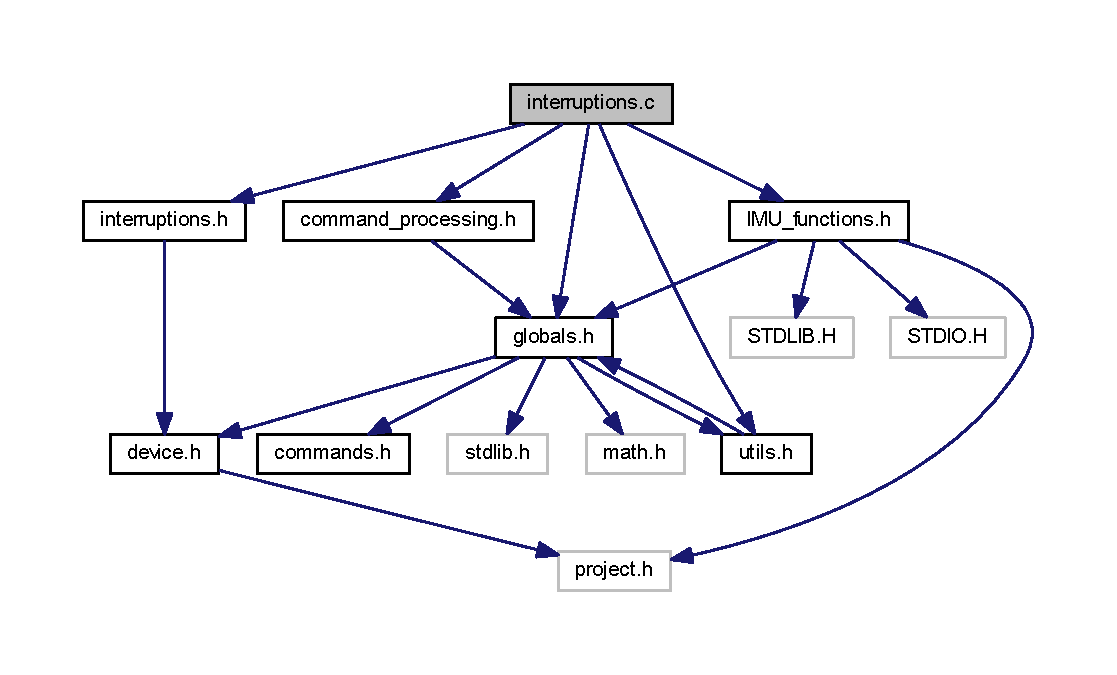
\includegraphics[width=350pt]{interruptions_8c__incl}
\end{center}
\end{figure}
\subsection*{Functions}
\begin{DoxyCompactItemize}
\item 
\mbox{\label{interruptions_8c_a7692d8c3185943c5bdfaa6de0a172ad3}} 
{\bfseries C\+Y\+\_\+\+I\+SR} (I\+S\+R\+\_\+\+R\+S485\+\_\+\+R\+X\+\_\+\+Ex\+Interrupt)
\item 
\mbox{\label{interruptions_8c_a9790811526002d99b25a814afd02cbae}} 
void {\bfseries interrupt\+\_\+manager} ()
\item 
\mbox{\label{interruptions_8c_a0fe51278c957933282ca63f3ac9beeaf}} 
void {\bfseries function\+\_\+scheduler} ()
\end{DoxyCompactItemize}


\subsection{Detailed Description}
Interruption functions are in this file. 

\begin{DoxyDate}{Date}
February 01, 2018 
\end{DoxyDate}
\begin{DoxyAuthor}{Author}
{\itshape Centro \char`\"{}\+E.\+Piaggio\char`\"{}} 
\end{DoxyAuthor}
\begin{DoxyCopyright}{Copyright}
(C) 2012-\/2016 qbrobotics. All rights reserved. 

(C) 2017-\/2018 Centro \char`\"{}\+E.\+Piaggio\char`\"{}. All rights reserved. 
\end{DoxyCopyright}

\section{interruptions.\+h File Reference}
\label{interruptions_8h}\index{interruptions.\+h@{interruptions.\+h}}


Interruptions header file.  


{\ttfamily \#include $<$device.\+h$>$}\newline
Include dependency graph for interruptions.\+h\+:
\nopagebreak
\begin{figure}[H]
\begin{center}
\leavevmode
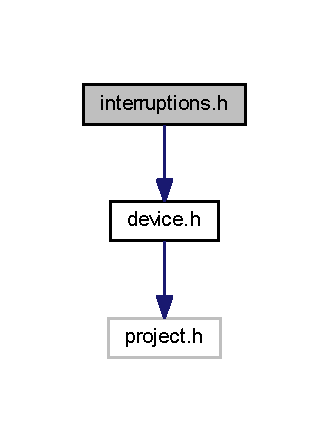
\includegraphics[width=158pt]{interruptions_8h__incl}
\end{center}
\end{figure}
This graph shows which files directly or indirectly include this file\+:
\nopagebreak
\begin{figure}[H]
\begin{center}
\leavevmode
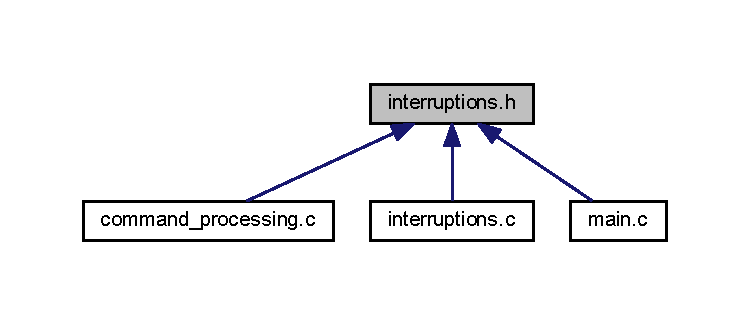
\includegraphics[width=350pt]{interruptions_8h__dep__incl}
\end{center}
\end{figure}
\subsection*{Functions}
\begin{DoxyCompactItemize}
\item 
\mbox{\label{interruptions_8h_a7e24af8c83537b0441877bf0f00dd30a}} 
{\bfseries C\+Y\+\_\+\+I\+S\+R\+\_\+\+P\+R\+O\+TO} (I\+S\+R\+\_\+\+R\+S485\+\_\+\+R\+X\+\_\+\+Ex\+Interrupt)
\item 
\mbox{\label{interruptions_8h_a0fe51278c957933282ca63f3ac9beeaf}} 
void {\bfseries function\+\_\+scheduler} ()
\item 
\mbox{\label{interruptions_8h_a9790811526002d99b25a814afd02cbae}} 
void {\bfseries interrupt\+\_\+manager} ()
\end{DoxyCompactItemize}


\subsection{Detailed Description}
Interruptions header file. 

\begin{DoxyDate}{Date}
February 01, 2018 
\end{DoxyDate}
\begin{DoxyAuthor}{Author}
{\itshape Centro \char`\"{}\+E.\+Piaggio\char`\"{}} 
\end{DoxyAuthor}
\begin{DoxyCopyright}{Copyright}
(C) 2012-\/2016 qbrobotics. All rights reserved. 

(C) 2017-\/2018 Centro \char`\"{}\+E.\+Piaggio\char`\"{}. All rights reserved. 
\end{DoxyCopyright}

\section{main.\+c File Reference}
\label{main_8c}\index{main.\+c@{main.\+c}}


Firmware main file.  


{\ttfamily \#include $<$device.\+h$>$}\newline
{\ttfamily \#include $<$globals.\+h$>$}\newline
{\ttfamily \#include $<$interruptions.\+h$>$}\newline
{\ttfamily \#include $<$command\+\_\+processing.\+h$>$}\newline
{\ttfamily \#include $<$utils.\+h$>$}\newline
{\ttfamily \#include $<$I\+M\+U\+\_\+functions.\+h$>$}\newline
Include dependency graph for main.\+c\+:
\nopagebreak
\begin{figure}[H]
\begin{center}
\leavevmode
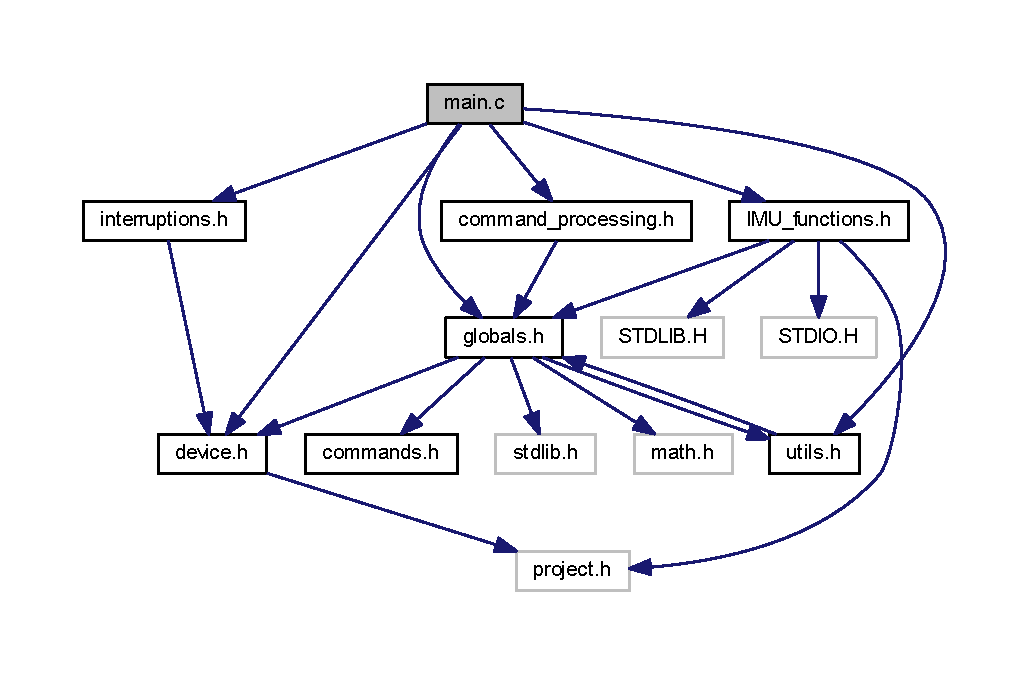
\includegraphics[width=350pt]{main_8c__incl}
\end{center}
\end{figure}
\subsection*{Functions}
\begin{DoxyCompactItemize}
\item 
\mbox{\label{main_8c_ae66f6b31b5ad750f1fe042a706a4e3d4}} 
int {\bfseries main} ()
\end{DoxyCompactItemize}


\subsection{Detailed Description}
Firmware main file. 

\begin{DoxyDate}{Date}
February 01, 2018 
\end{DoxyDate}
\begin{DoxyAuthor}{Author}
{\itshape Centro \char`\"{}\+E.\+Piaggio\char`\"{}} 
\end{DoxyAuthor}
\begin{DoxyCopyright}{Copyright}
(C) 2012-\/2016 qbrobotics. All rights reserved. 

(C) 2017-\/2018 Centro \char`\"{}\+E.\+Piaggio\char`\"{}. All rights reserved. 
\end{DoxyCopyright}

\section{utils.\+h File Reference}
\label{utils_8h}\index{utils.\+h@{utils.\+h}}


Definition of utility functions.  


{\ttfamily \#include $<$globals.\+h$>$}\newline
Include dependency graph for utils.\+h\+:
\nopagebreak
\begin{figure}[H]
\begin{center}
\leavevmode
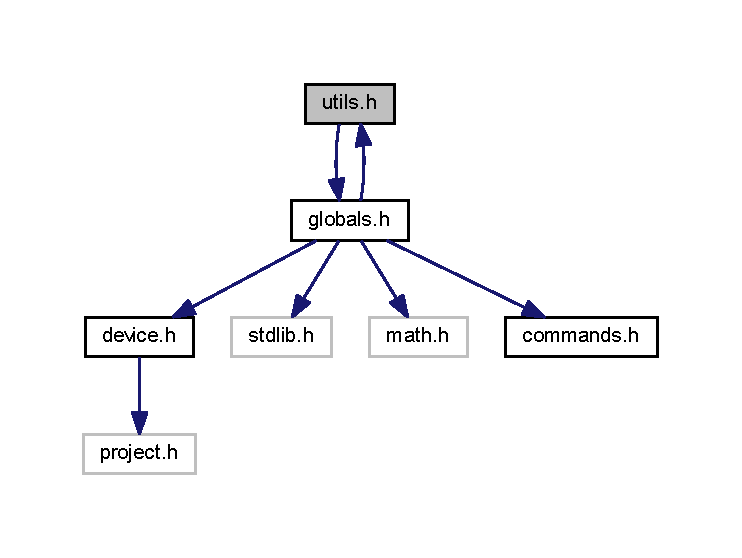
\includegraphics[width=350pt]{utils_8h__incl}
\end{center}
\end{figure}
This graph shows which files directly or indirectly include this file\+:
\nopagebreak
\begin{figure}[H]
\begin{center}
\leavevmode
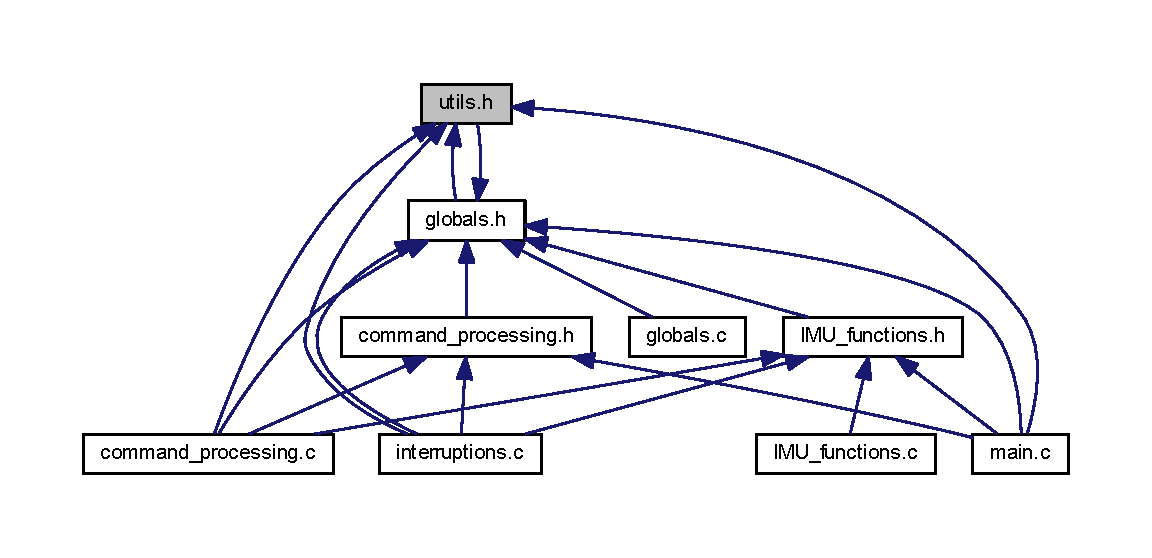
\includegraphics[width=350pt]{utils_8h__dep__incl}
\end{center}
\end{figure}
\subsection*{Functions}
\begin{DoxyCompactItemize}
\item 
\mbox{\label{utils_8h_a5e5346796220b271615a52428f6ec6ca}} 
float {\bfseries inv\+Sqrt} (float x)
\item 
\mbox{\label{utils_8h_a88d150c696b69e576a1dfb193266ae6a}} 
void {\bfseries v3\+\_\+normalize} (float v3\+\_\+in[3])
\item 
\mbox{\label{utils_8h_a2965058da02ba33e26af00cff2fcfec2}} 
void {\bfseries v4\+\_\+normalize} (float v4\+\_\+in[4])
\end{DoxyCompactItemize}


\subsection{Detailed Description}
Definition of utility functions. 

Declaration of utility functions.

\begin{DoxyDate}{Date}
February 01, 2018 
\end{DoxyDate}
\begin{DoxyAuthor}{Author}
{\itshape Centro \char`\"{}\+E.\+Piaggio\char`\"{}} 
\end{DoxyAuthor}
\begin{DoxyCopyright}{Copyright}
(C) 2012-\/2016 qbrobotics. All rights reserved. 

(C) 2017-\/2018 Centro \char`\"{}\+E.\+Piaggio\char`\"{}. All rights reserved.
\end{DoxyCopyright}
\begin{DoxyDate}{Date}
February 01, 2018 
\end{DoxyDate}
\begin{DoxyAuthor}{Author}
{\itshape Centro \char`\"{}\+E.\+Piaggio\char`\"{}} 
\end{DoxyAuthor}
\begin{DoxyCopyright}{Copyright}
(C) 2012-\/2016 qbrobotics. All rights reserved. 

(C) 2017 Centro \char`\"{}\+E.\+Piaggio\char`\"{}. All rights reserved. 
\end{DoxyCopyright}

%--- End generated contents ---

% Index
\backmatter
\newpage
\phantomsection
\clearemptydoublepage
\addcontentsline{toc}{chapter}{Index}
\printindex

\end{document}
